\documentclass{sig-alternate}
\usepackage{enumitem}
\usepackage{xspace}
\usepackage{caption}
\usepackage{subfig}
\usepackage{paralist, tabularx}

\begin{document}
\newcommand{\nifty}{\textsf{Papyr}\xspace}

\conferenceinfo{DEV}{'14 San Jose, California USA}
\title{Papyr: Automatically Generating ``Smart" Paper Tools for Low-resource Settings}
\author{}
\maketitle

\begin{abstract}

Despite the recent push toward leveraging information and communication technologies (ICTs) to replace paper-based tasks, there remain many barriers to designing appropriate and deployable technical solutions that replace paper.
As a result, paper tools such as forms, charts, and graphs continue to be widely used in low-resource organizations working in developing regions.
Unfortunately, existing paper tools are often designed to be out of reach for end-users and depend on intermediaries to input data and interpret information. 
We apply ideas from computability and human-computer interaction to design a system that automatically generates paper tools to provide immediate computational and visual feedback as well as independence from both ICTs and intermediaries at the point of use. 
\nifty is a system that is easy to use and allows low-resource organizations to quickly transform data tracking or information dissemination requirements into printable ``smart'' paper tools. 
In this paper, we explore how paper tools are currently being used by organizations in Ghana, explore the design space for smart paper tools, and describe \nifty's design and implementation.

\end{abstract}

% \category{}{}{}
% \category{}{}{}
% \terms{}
% \keywords{}

%%%%%%%%%%%%%%%%%%%%%%%%%%%%%%%%%%%%%%%%%%%%%%%%%%%%%

\section{Introduction}


Even as computing devices proliferate and attempt to eliminate paper from a given ecosystem, it is undeniable that paper continues to be pervasive in professional and personal spaces.
Paper is light, low-cost, familiar, accessible, easy to use, intuitive to manipulate, and convenient to distribute \cite{sellen1997,sellen2002,johnson1993}. Moreover, in low-resource settings where technology infrastructure such as stable electricity, cutting-edge computer hardware and software, and skilled human capital is deficient, paper is an obvious choice because it can accomplish many of the same tasks that computers can. Furthermore, generations of paper-based organizational and end-user tasks have ensured that national regulations seek compliance with paper-based record keeping rules. The enduring legacy of paper, especially amongst current paper-based workflows, provides inertia against switching to more technically intensive replacements. 

Still, paper is not without its constraints. When compared to information and communication technology (ICT) alternatives, paper is less malleable once data is inscribed, has less ``computational output'', and is difficult to digitize. Electronic media that is designed and built to replace paper possesses an inverse profile of not only strengths, but also constraints, unable to capitalize on paper's accessiblity and tangiblity \cite{johnson1993}. Can paper itself be designed to overcome some of its limitations? Can paper, for instance, make its static content dynamic? Or, perhaps, more ambitiously, provide computational feedback to its end users?

There already exist many examples of ``smart paper'' that demonstrate how these lofty objectives are in fact possible. Paper graphs, for instance, can provide computational feedback. The nomograph has three scales that represent a three-variable equation. In one illustration, plotting along these scales with just a pen can determine ideal body mass within the ``overweight", ``desirable", or ``underweight" categories, while taking gender into account \cite{thomas1976}. The partograph, another example, is a graphical tool that can provide predictive feedback to doctors or midwives throughout the progress of labor \cite{who1988}. It is popular in low-resource settings, a cost-effective and accessible tool that when coupled with well-defined protocols and appropriate instruction has been shown to demonstrate distinct benefits \cite{fawole2009, umezulike1999, fahdy2005, pettersson2000}.

These examples of ``smart" paper tools indicate a particularly compelling research problem of leveraging paper's many useful properties and developing more standalone tools, validating their usefulness in low-resource settings where paper is cheaper, more familiar, and more accessible than its technological counterparts. Our study addresses this research problem and explores the ``smart'' paper space with the following contributions:

\begin{compactitem}

  \item Needs assessment of low-resource settings for microfinance and health in Ghana through an appraisal of existing paper artifacts and understanding of information needs. (Section~\ref{sec:exploring-paper}).
  \item Development of ``smart'' paper tools design iterations through brainstorming sessions and in the field feedback to push the boundaries of paper, especially with low-resource settings and low-literate populations in mind (Section~\ref{sec:exploring-paper}).
  \item Discovery of basic design principles that highlight the constraints of paper and user interaction with ``smart'' paper tools (Section~\ref{sec:constraints}).
  \item Construction of \nifty, a system for intermediaries from low-resource organizations to automatically generate ``smart'' paper tools by defining their tasks and their associated paramters and selecting from suggestions based on resources available and capabilities of the end-user (Section~\ref{sec:system-desc}). 

\end{compactitem}

%%%%%%%%%%%%%%%%%%%%%%%%%%%%%%%%%%%%%%%%%%%%%%%%%%%%%

\section{Related Work}
\label{sec:related}

% \emph{The spectrum between paper and technology.} 
There is a spectrum of innovations that attempt to bridge the gap between technology and paper and leverage the benefits of both, a spectrum based on the degree of integration with technology, as described in Figure~\ref{fig:spectrum}.

\begin{figure}
\centering

\includegraphics[width=\linewidth]{img/spectrum.png}
\caption{Spectrum between paper and technology (Section~\ref{sec:related})based on the degree of integration with technology: leftmost end is most tightly coupled with technology and rightmost is most free of technology.}
\label{fig:spectrum}
\end{figure}

The tools that rest in the space between paper and technology most strongly integrated with technology are \emph{paper-like technologies}. This includes a set of tablets and mobile devices, including PaperTab, PaperFold, and MorePhone, that are electronic devices as reconfigurable as paper itself \cite{gomes2014,gomes2013,tarun2013}. The selling point of these technologies are their paper-like properties, including portability, maneuverability, and flexibility, creating a familiar look and feel to technology with the same capacities as a full-fledged tablet or phone. This reinforces the draw to include the benefits of paper in technological design, but does so in a fairly expensive way.

Other tools attempt to explore the role of paper documents as interfaces to the digital world, or the field of \emph{paper computing} \cite{kaplan2010}. This includes systems that use paper to control technological environments, such as Digital Desk, the projection of graphics interfaces on a paper-based workspace, or PaperPoint, the control and annotation of PowerPoint presentations using printed slide handouts \cite{newman1992,wellner1993,signer2007}. In addition, this includes tools that provide technological links to paper, such as printed visual markers (QR codes and barcodes); specialized devices for annotations and digitally inputted notes; computer vision based digitization of paper; and cloud computing \cite{kaplan2010,anoto,pietrzak2010}. However, these technologies often use paper as an aid to technology as opposed to utilizing paper's beneficial properties on its own. 

Paper can be used to model technology in paper prototyping or paper composites. \emph{Paper prototyping} utilizes paper's accessibility and ability to be easily manipulated to simulate and test the usability technological designs in a ``wizard of oz'' experimental structure \cite{synder2001,chandler2002}. While technology is not integrated in the creation of the tool, the tool is paradoxically dependent on technology because it has no power when used alone. On the other hand, \emph{paper composites}, or combinations of paper with technological materials, such as the paper and conductive thread combination in pulp-based computing, can give these paper-based tools more power, but still exist to simulate technology and are reliant on technological components \cite{coelho2009}.

% \emph{Paper and technology in low-resource settings.} 
One of the problems with this type of relationship with technology and technological components in the workflow is cost and a reliance on tools and materials that low-resource organizations do not necessarily have. However, there are some innovations that attempt to bridge the gap between existing paper materials with low-cost technological interfaces like mobile phones.

Looking specifically at some tools developed for low-resource settings, most are tightly reliant on technology and fall in the \emph{paper computing} category. There are tools that recapture information on paper into the technological space, such as CAM, which uses a camera to record and store data from paper logs in rural microfinance groups in India; ODK Scan, which applies computer vision techniques on small ``snippets" of the content for a single form field; and Shredder, a combination of computer vision, database, and crowdsourcing techniques to transmit and verify information from paper forms \cite{parikh2006, akona2009, dell2012, dell2013, chen2012}. There are also tools that use technology to track the actual process for data input on paper-based forms such as Digital Slate, which uses the pen to paper writing motion to capture data in savings groups in India, and Partopen, which is a digital pen specifically developed for filling out the partograph in maternal labor \cite{ratan2010, underwood2012, underwood2013}. And there are even tools that use a mix of technology and paper in the information gathering process itself, such as Local Ground, a barcoded geospatial surveying tool \cite{wart2010}.

In addition to being tightly coupled with technology, these tools are used mainly for information collection, including both retroactive and active data capture. They do not give very much feedback to the user at the time of use and thus does not leverage one of the important components of computation.

We believe \nifty is an unusual but appropriate marriage between paper and technology for developing contexts: a computer is used to support the organization's design of context-specific paper tools, but the produced paper tools require no ICT support or leverage at the end user. Moreover, \nifty provides feedback to the end-users, encouraging utilization and adherence to the processes.

%%%%%%%%%%%%%%%%%%%%%%%%%%%%%%%%%%%%%%%%%%%%%%%%%%%%%

\section{Exploring Paper}
\label{sec:exploring-paper}

After reviewing related work and identifying real-world problems in the health and microfinance contexts in low-resource settings where paper is already deeply rooted and in constant use, we developed two sets of design iterations: one based solely on brainstorming sessions (Section~\ref{sec:brainstorming}) and the other based on in the field feedback from health and microfinance field sites in Ghana (Section~\ref{sec:field}). 

\subsection{Brainstorming Design Iterations}
\label{sec:brainstorming}

The primary goal of these preliminary brainstorming sessions was to push the boundaries of what ``smart paper" could accomplish. In other words, how could we re-design paper in a way that makes it somehow better? Here, we describe a small subset of the ``smart-paper" tools we designed.

\subsubsection{The Subtraction Band}
\label{sec:subtraction}

\emph{Use case.}
One problem in the microfinance domain for low-literate users is tracking exactly how much is earned and where money is spent in a given day. We design a tool that helps tackle one source of difficulty for this problem: doing addition and subtraction of expenditures.

\emph{Proposed tool.}
The base is made of stiff paper, plastic, cardboard, or other material that could support two narrow slits through which a closed paper loop could be smoothly slid and rotated. There are two sections on the base, the top section is a basic scale of amounts with a predetermined interval and the bottom is the band threaded through two slits. This band can be made with paper or waxed paper to ensure smoother sliding. A depiction can be seen in Figure~\ref{fig:band}.

% \textbf{Usage.}
An individual will place a sticker in each slot every time they earn money that day. To take a simple example, say an individual has earned cumulatively 10 cedi\footnote{local currency corresponding to roughly 0.28 USD per cedi at the time of writing} today. The band is marked up to the 9th slot. However, the individual now spends 3 cedis. They will remove the stickers up to the 3rd slot. Then, they can shift the band to the left such that the first filled slot moves back to the leftmost point, or the 1st slot.
The individual can opt to shade in the band instead of using stickers.

\emph{Lessons learned.}
This tool can be generalized from the basic use case to include any type of task that requires addition and subtraction. 

\begin{figure}
\centering
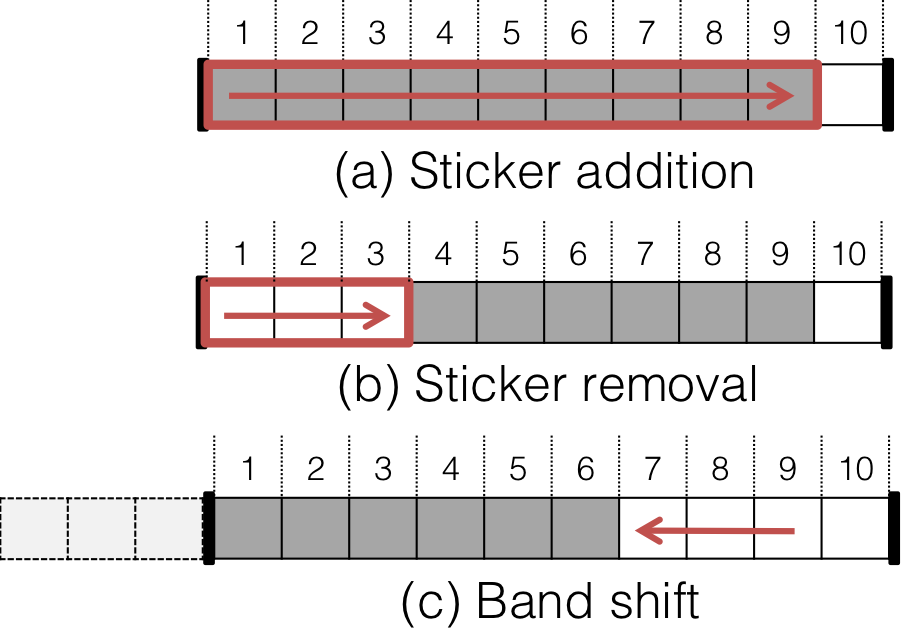
\includegraphics[width=.6\linewidth]{img/band.png}
\caption{\emph{Subtraction band (Section~\ref{sec:subtraction})}. First populate the band with stickers to obtain the sum of cumulative addition (a). Then remove stickers up to the amount that is being subtracted (b). Finally, slide the band so the stickers line up with the start and the resulting difference (c).}
\label{fig:band}
\end{figure}

\subsubsection{The Addition By Matching Tool}
\label{sec:add}

\emph{Use case.} Low-income populations are typically engaged in the informal labour market, meaning their income inflows are irregular and variable, accumulated through a variety of financial instruments such as earnings from jobs and borrowing from sources of credit. We decide to design a tool that can check if expenses exceed incomes and allow the user to flexibly update any changes in projected values.

\emph{Proposed tool.} Again, the base is made of stiff paper, plastic, cardboard, or other material that supports two narrow slits through which a paper strip could be smoothly slid up or down. Figure~\ref{fig:add} is a representation of this tool. The horizontal axes indicates where each separate strip is strung and the vertical axes indicate the amounts accumulated on each strip.

% \textbf{Usage.} 
If a user estimates that the incomes for the first day will be around 20 cedi, she or he fills the cells in the income column for Day 1 up to the 20 cedi mark on the vertical axis. And then if the user estimates that on the second day, the income will be approximately 30 cedi, she or he fills the cells up to the 30 cedi mark on the axis and then shift the band so that the stickers start after the filled income for the previous day, the 20 cedi mark. The user can then easily tell that over the two days, the income has been accumulated to 50 cedis. The user then can finish populating the rest of her or his projected income in a similar manner and continue in a similar manner for the expenses columns. In the example, the user can then see that over three days, she or he as earned and spent cumulatively 60 cedis. The user can also see that expenses exceed income on Day 1, income exceeds expenses on Day 2, and match on Day 3.

While tracking incomes and expenses, if there is an unexpected 10 cedis of expense that is introduced on Day 1, then the successive stacks of expenses must be readjusted. This is achieved by sliding the paper strip for the expenses on the following day up so that the filled in units rest above the end of the filled units for the day that was altered, and continued through to all of the successive days.

\emph{Lessons learned.} This tool can be generalized to calculate any cumulative sum and compare and match analogous variables.

\begin{figure}
\centering
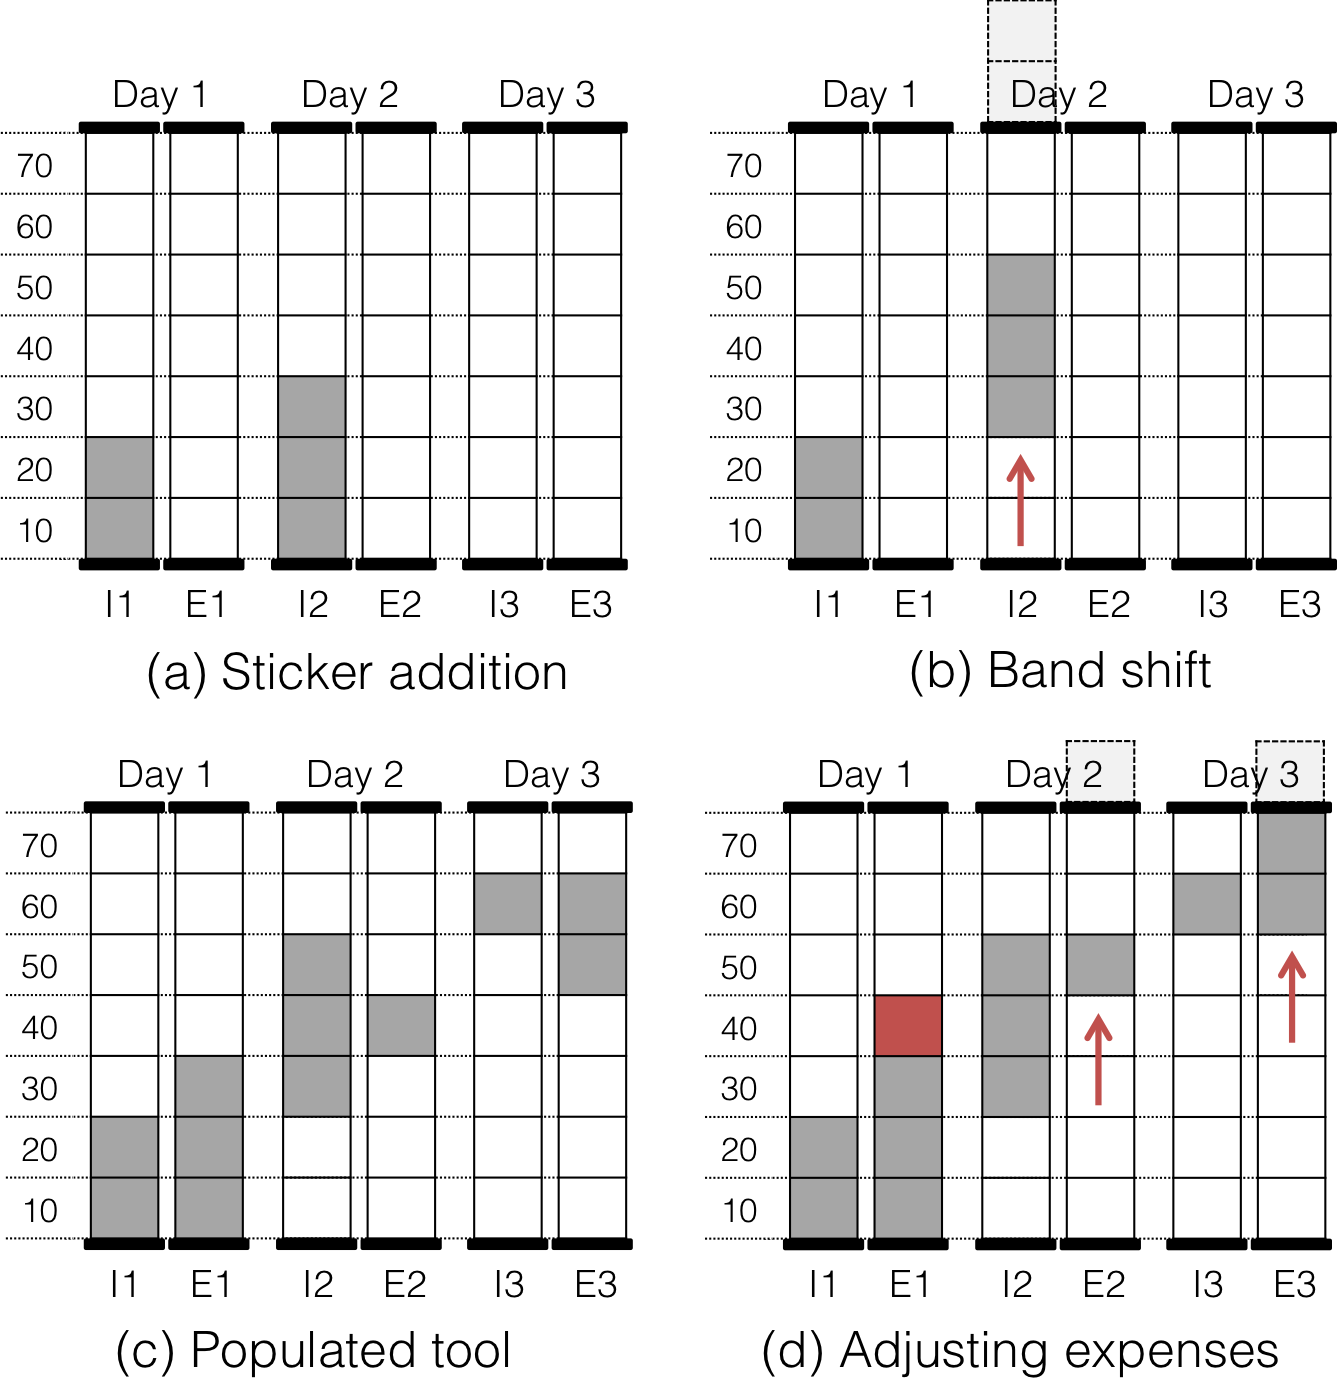
\includegraphics[width=.9\linewidth]{img/add.png}
\caption{\emph{Addition by matching tool (Section~\ref{sec:add})}. Populate each of the columns based on the scale on the y-axis (a) and shift the bands that so that their stickers stack above those of the previous band (b), see an example of a completed tool (c). In the case of an additional expense, adjust the bands that follow to maintain the ``stacked'' invariant (c).}
\label{fig:add}
\end{figure}

\subsubsection{Averages Tool}
\label{sec:average}

\emph{Use case.} 
Often times in villages, women do not actively tracking their menstrual cycle, making it hard to know when ovulation is likely to occur and when she is most fertile or if she has missed her period and is pregnant. We create a tool to help women track their menstrual cycles to give them a sense of their average cycle length.

\emph{Proposed tool.}
In its simplest form, the tool is a long strip of paper segmented to represent different days. Every seven segments, the strip is highlighted with a different color to indicate the beginning of a week.

% \textbf{Usage.}
Each day the individual does not have their period, she will unroll the strips of paper. 
On the day the woman does get her period, she will rip the strip of paper at that point to get a segment of dates that represent that one cycle. Once there are paper sections for each of the cycles, these sections are arranged next to each other. This could give a good ``eyeball'' estimate of the average, and the woman can have a sense of where the average lies, as seen in the dotted region in Figure~\ref{fig:average}(a). The next time, as the the woman is unrolling her strip of paper, she will know that as her paper lines up similarly to the previous cycles, she should anticipate to be her period. This could be enhanced with the use of a tool that lines up with the shortest strip and the longest strip in the range of data points and, with springs or rubber bands attached to the middle mark, draws a line between the two to come up with an alternate means of estimating the average. This is seen with the bars and coils in Figure~\ref{fig:average}(b).

Figure~\ref{fig:average}(c) and (d) depicts a different design iteration for determining averages is the wrapping method. The woman still continues to unroll the strips each day that she does not get her period. However, she will not rip the strips of paper on the days that she does get her period. Instead, she will have a length of the strip that represents all of the cycles she has had from the beginning. In this example, the woman has a strip with the length of 167 for her 6 cycles. Then, she will take this long strip and wrap it around two rods, potentially pencils, the number of times she has her cycles. In this example, she has had 6 cycles, so she will wrap the strip tightly six times around the two rods while tracking the end of the 167 day length. She can then hold onto the rods and separate them in a parallel manner in opposite directions until one rod is lined up with the square for the first day and the other rod is lined up with the square for the last day. This should give an even six lengths for the 167 days, which represent the average of the days.

\emph{Lessons learned.}
The strips of paper with date increments can be used for any type of time or date tracking. And the methods of comparing these date strips can be used for any type of averages tracking. 

\begin{figure}
\centering
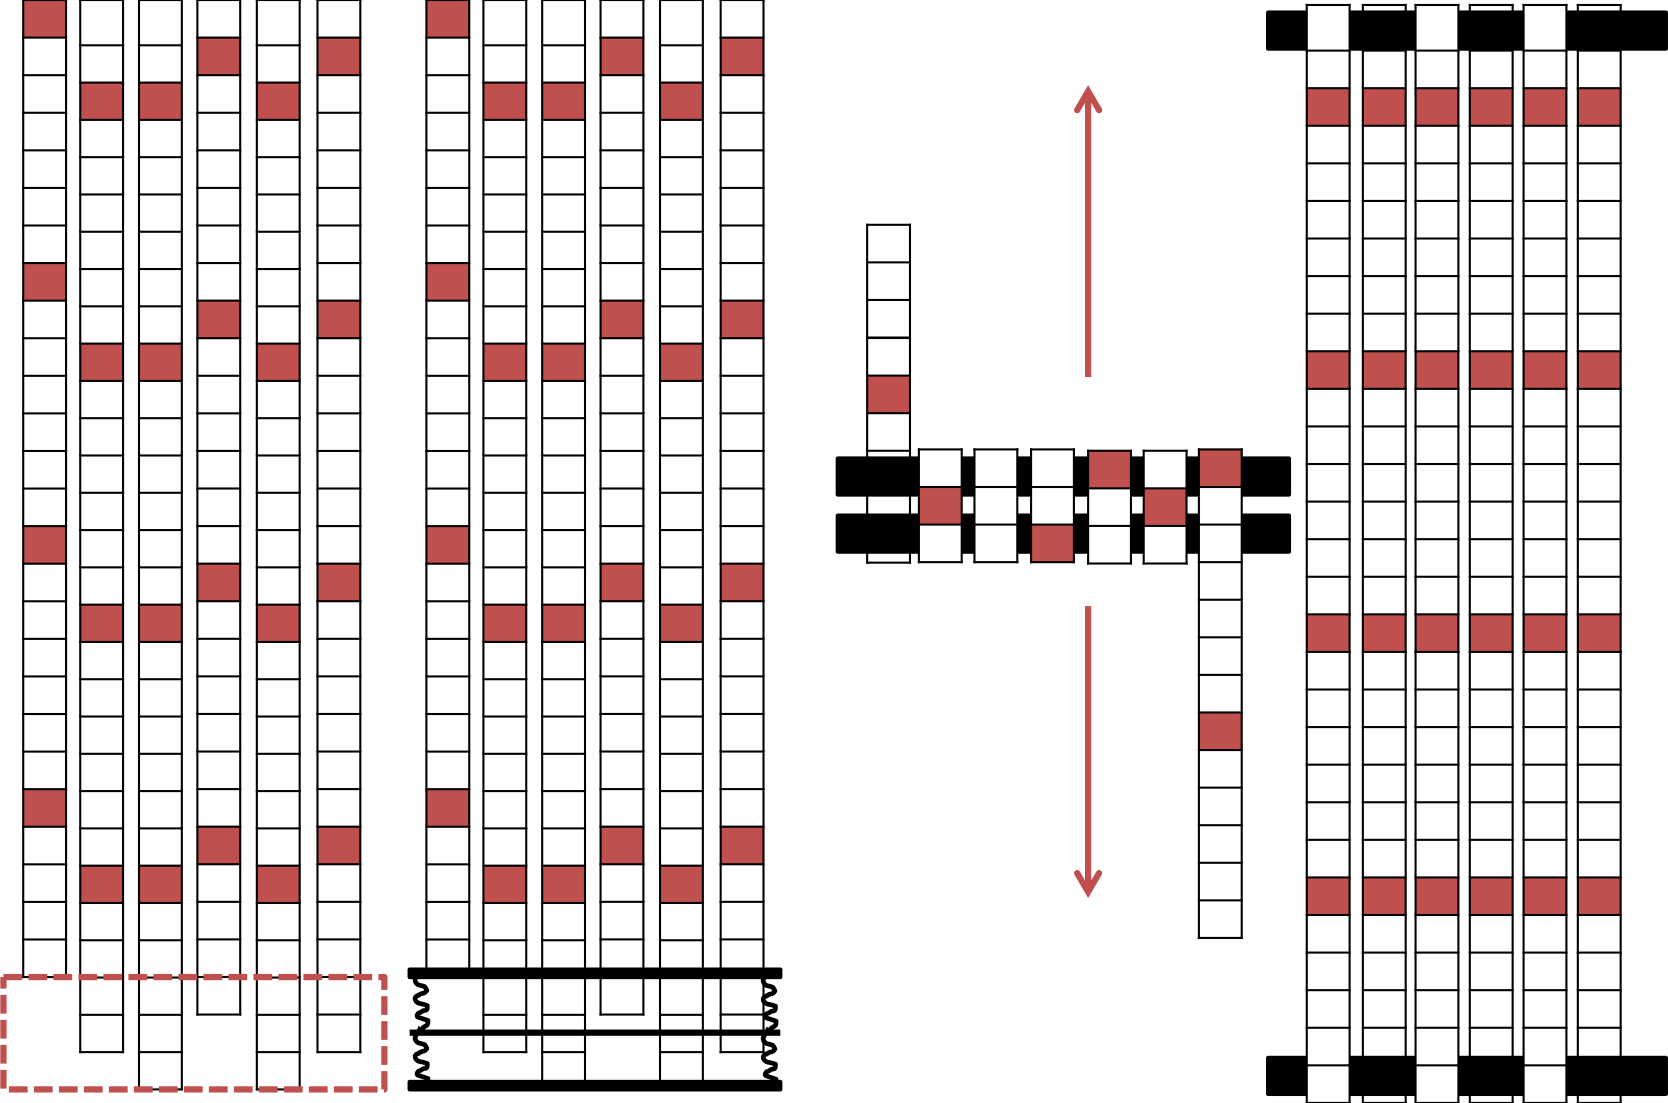
\includegraphics[width=\linewidth]{img/average.png}
\caption{\emph{Averages tool (Section~\ref{sec:average})}. To find the average of a series of section lengths, line them up next to each toehr and visibly estimate the average length (a) or use a tool to find the midpoint between the shortest and longest lengths (b). Alternatively, instead of separating into sections, take the full strip and wrap it around two rods the number cycles (c) and slowly pull the two rods apart to have the entire length be separated evenly (d).}
\label{fig:average}
\end{figure}

\subsection{In the Field Design Iterations}
\label{sec:field}

We conducte contextual inquiries in the domains of microfinance and public health in the Greater Accra region in Ghana, including Tema, Dodowa, and Awutu, over a period of three weeks in July 2014. During this time, we observe the organizational settings, user practices, and existing paper artifacts. 

\subsubsection{Susu Tracker}
\label{sec:susu}

\emph{Use case.}
We spent time with a microfinance institution (MFI) in Tema, observing their daily ``susu" (savings) operations. Clients deposit a standard amount for 31 days where 1 day is kept by the MFI as commission. These transactions are logged in a standard paper passbook (Figure~\ref{fig:susu}(a)) along with the date on which a deposit was made, the amount deposited, and the running total for each cycle. However, the amount taken for commission and the cumulative sum across different cycles is not provided by the passbook. Therefore, when the customer goes for a withdrawal, they are unaware of how much money they have saved up in total and how much of the money they put in was separated for commission. We designed a tool that could give the customer this missing information, specifically geared toward those with low-literacy and arithmetic skills.

\emph{Proposed tool.}
We tested the usability of five design iterations with existing customers. 
The first iteration is a calendar with a stack of stickers that has the running total, with commission accounted for in the first deposit of a cycle by a red sticker (Figure~\ref{fig:susu}(b)). The final iteration utilizes no stickers, but, in a simple passbook format, has the running total over all of the different cycles already printed out in the overall balance column (Figure~\ref{fig:susu}(c)). 

% \textbf{Usage.}
\emph{Lessons learned.}
With the feedback from the users, it was found that the layout that capitalizes on the familiarity of the existing passbook format and required the least amount of additional materials (ie, using only a pencil vs. a separate stack of stickers) is the most effective.


\begin{figure}
\centering
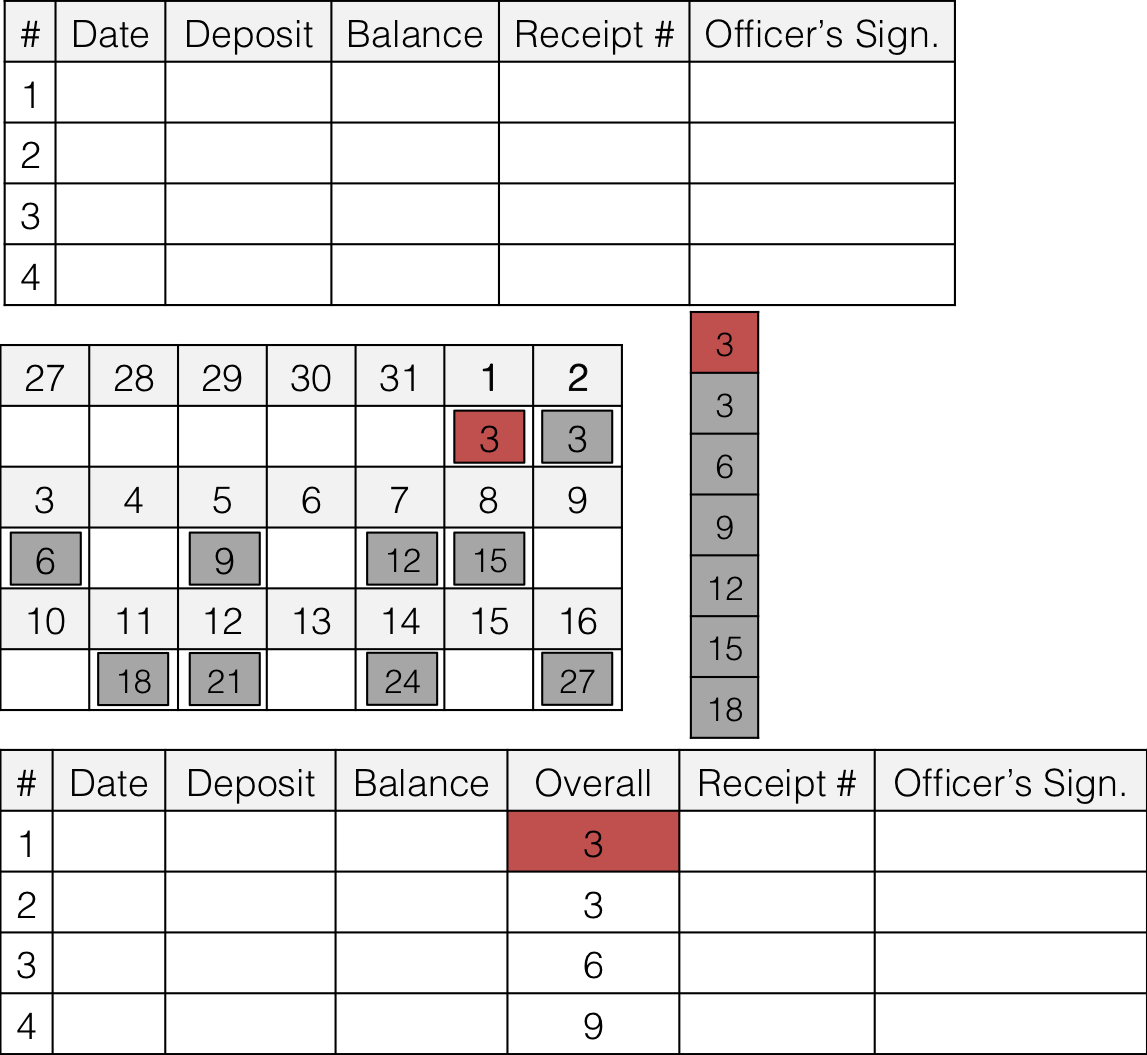
\includegraphics[width=.75\linewidth]{img/susu.png}
\caption{\emph{Susu tracker (Section~\ref{sec:average})}. A basic passbook (a) can be improved to show commission and cumulative sum information by using a calendar and sticker tracker (b) that has preprinted sums on the stickers or a simpler augmented passbook that has the cumulative sum prepopulated (c).}
\label{fig:susu}
\end{figure}

\subsubsection{Graph Reader}
\label{sec:graph}

\emph{Use cases.}
We observed medical practices and conducted interviews with different doctors and nurses at government district and children's hospitals in the greater Accra region. We also interviewed medical professors and intermediaries, such as local community health volunteers. 

There is a chart that nurses use to determine whether the child is at a healthy weight-age balance based on the WHO regulations of child growth percentiles. This chart also tracks the child's weight over 24 months, accompanied by a legend to indicate the possible slopes between each of the points, and their implications, as seen in Figure~\ref{fig:graph}(c). Though this information is relevant to the mothers, the confusing and esoteric presentation makes it inaccessible for those who do not know how to read graphs, and clunky to use for those who can. Therefore, we decide to develop a tool that helps individuals read this graphical information more easily.

\emph{Proposed tool.}
% \textbf{Usage.}
To improve this tool for low-literate populations, the first challenge is pinpointing the location of the information of interest. Various ideas for tools were developed, including hollow strips that overlap to box a specific region in the center and tabs that stretch to the numbers of interest on the graph and position the basic square viewfinder (Figure~\ref{fig:graph}(a)).However, based on design principles for low-literacy users and feedback from the needs assessment, we to not only highlight the important regions but also cover the information that is not needed. Therefore, with overlapping pages we developed a tool that uses horizontal and vertical tabs to slide the region of emphasis in place. An example of this tool can be seen later in the paper in Figure~\ref{fig:graph}(b).

Another design question is finding ways to compare two points with each other. This could involve something as basic as the slope comparison that the current child and maternal health records use. Or, this could use the viewfinder's space to compare the slope of two points. After feedback from nurses and doctors, the final iteration of the tool includes a viewfinder that compares points based on the quadrants they fall in, as seen in Figure~\ref{fig:graph}(d).

\emph{Lessons learned.}
We find that the tools that have a narrower field of view and focus on the important information are most effective. Additionally, having a simple viewfinder can help increase the computational feedback provided by the paper graphs. 
These graph reading enhancements can be applied to any type of basic line graph. 


\begin{figure}
\centering
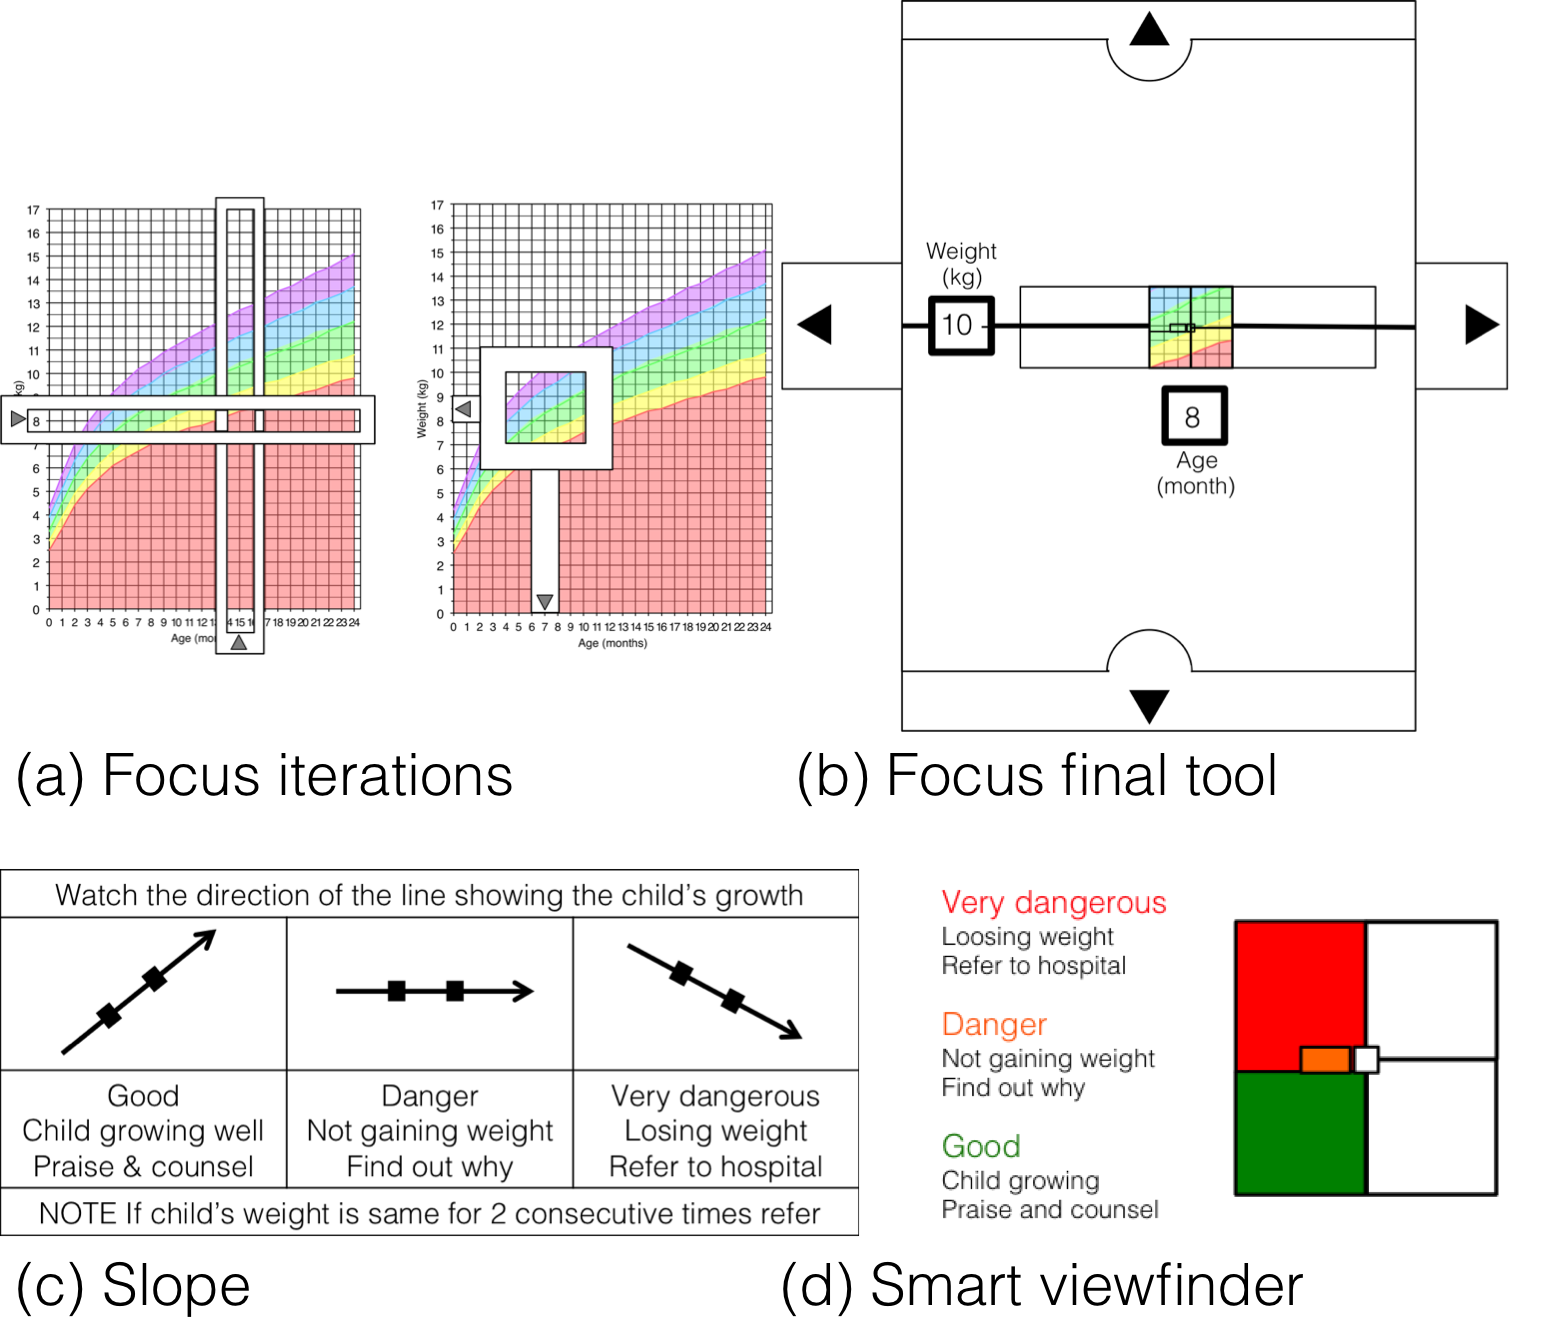
\includegraphics[width=\linewidth]{img/graph.png}
\caption{\emph{Graph reader (Section~\ref{sec:graph})}. Different contenders for trying to focus on the important information in the graph include hollow strips and a basic square (a) but the final tool is based on horizontal and vertical sliding tabs (b). Comparing two points is possible using positive, negative, and zero slopes (c) or a smart viewfinder sectioned into corresponding quadrants (d).}
\label{fig:graph}
\end{figure}

\subsubsection{Flowchart Booklet}
\label{sec:flowchart}

\emph{Use cases.}
Through interviews with a reputable nonprofit organization engaged in public health interventions and interactions with community health volunteers, we learned that one of the tools used by nurses is a decision tree for diagnosing common ailments. This is derived from the Integrated Management of Childhood Illnesses (IMCI), which is a flowchart that instructs the intermediary which symptoms to check for or questions to ask and how to proceed depending on the results of these inquiries. However, the current representation of the logic for this process is too overwhelming with a lot of detailed information or simplifications to accommodate information in a single diagram. Therefore, we decide to create a more efficient tool for presenting this information.

\emph{Proposed tool.}
We started by simplifying the flowchart so that each potential option is represented by a different sections of the pages of the booklet (Figure~\ref{fig:flowchart}(a)). However, we soon found that this decreases the amount of space that we have on the page and detract from our ability to properly show all of the information. So we decided to use tabs to demonstrate the options that a user could take at a given point. After demonstrating our first iterations to an audience of doctors and nurses, it was found that the movement from one step to another was not self-explanatory. Even though the users follow the steps on the booklet, it was difficult to know when to stop. We tried adding arrows to the pages to indicate the flow from one page to the next, but the arrows were unclear when it came to needing to choose which option to flip. Finally, we found that we need to make the options more clear but also to append a long red bar that said ``STOP" at the end of a given action sequence, as seen in Figure~\ref{fig:flowchart}.

% \textbf{Usage.}
\emph{Lessons learned.}
We find that since any ``smart" paper tool in a low-resource setting will most likely not come with many user instructions or training sessions, the progression from one step to another has to be fairly clear to the user.

\begin{figure}
\centering
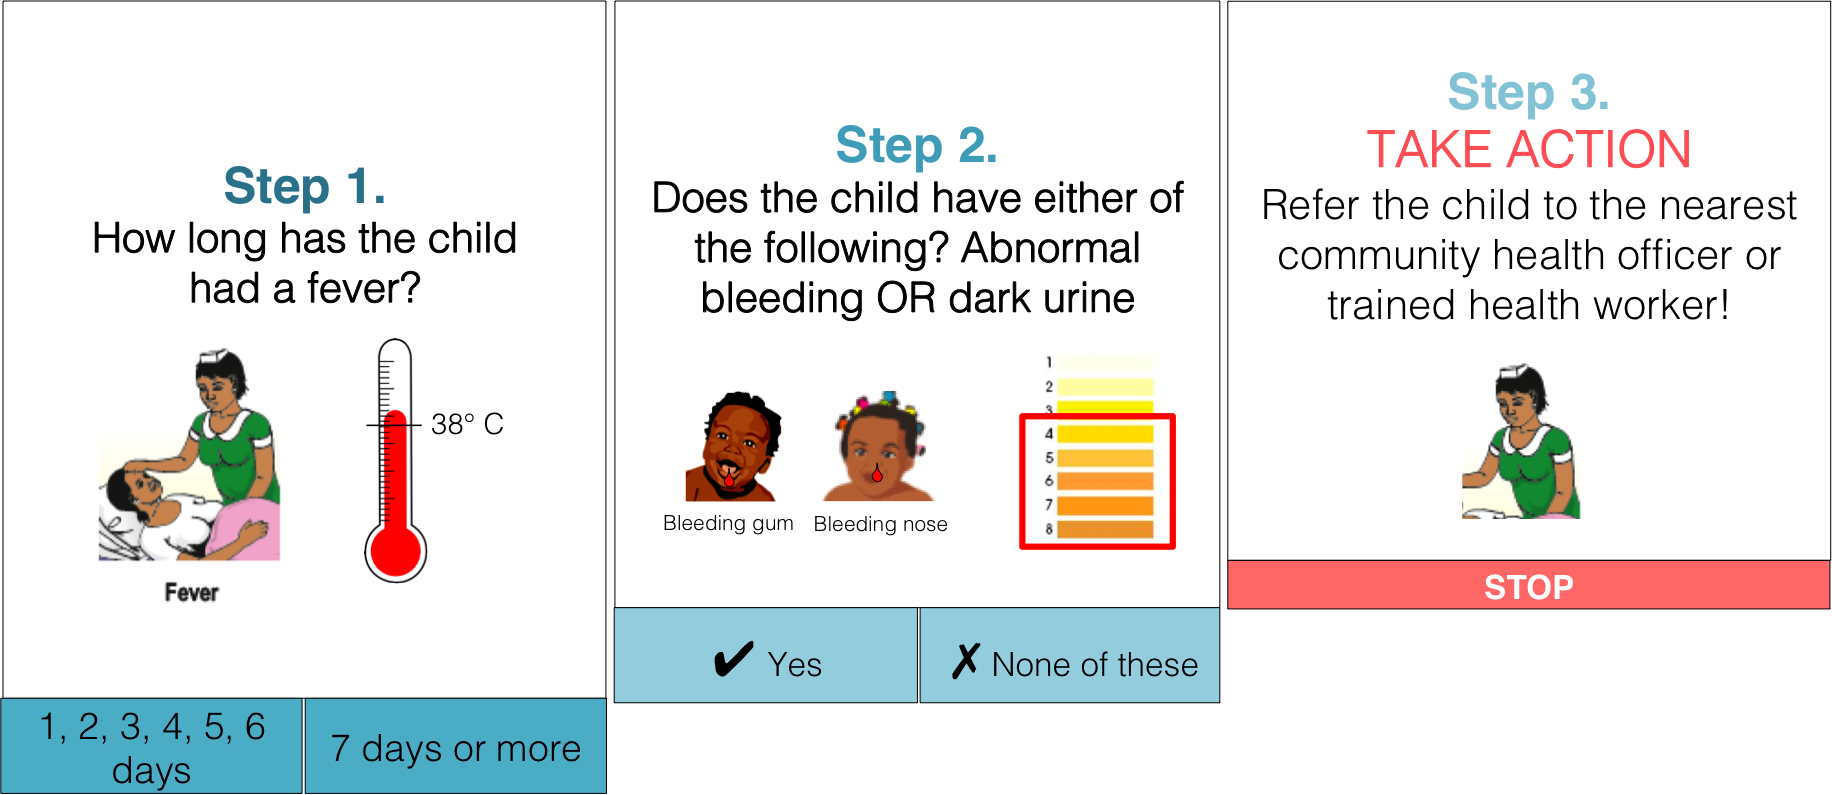
\includegraphics[width=\linewidth]{img/flowchart.png}
\caption{\emph{Flowchart booklet (Section~\ref{sec:flowchart})}. The first iteration had each option as a separate part of the page (a) but the final iteration uses tabs for the options (b).}
\label{fig:flowchart}
\end{figure}

%%%%%%%%%%%%%%%%%%%%%%%%%%%%%%%%%%%%%%%%%%%%%%%%%%%%%

\section{Design Constraints}
\label{sec:constraints}

% Given the immense design space of paper-based tools we had to limit our scope for this project. 
% We reflected upon the paper tools that we encountered and explored in order to abstract our ideas into basic primitives that could be shared across tools. 
% Here we consider the various constraints of paper itself, our target users, and our specific contexts to scope the eventual design of \nifty.

%\subsection{Paper Primitives}
%\label{sec:abstraction}

%Reflecting upon some of the paper tools that were encountered and developed, we found that there were some ideas that were common across several of the paper-based tools. For example, both the decision tree tool and the graph reading tool engage different techniques try to narrow the focus so that the end user is dealing with only the information that is relevant to a given scenario. The decision tree tool does so by placing each of the steps or questions on a separate page and the graph reading tool does so by blocking the graph except for the section relevant to the end user. Each of these properties can be traced back towards a more basic aspect of interacting with a two-dimensional piece of paper. In the previous example, both of the tools utilize layering of pages to obscure the irrelevant information and highlight or focus on the currently important information. These aspects such as layering could be considered paper \textit{primitives} that provide specific types of feedback to the user. A list of some examples of primitives and their associated feedback can be found in Table~\ref{table:primitives}.

%\begin{table*}
%\centering
%\caption{Paper primitives and their feedback}
%\begin{tabular}{|p{.35\linewidth}|p{.6\linewidth}|} \hline
%% \being{tabular}{|l|l|} \hline
%\textbf{Primitive} & \textbf{Feedback} \\ \hline
%Color & Highlighting a concept, categorizing an input \\ \hline
%Writing (tallying, words, numbers) & Marking when an event occurs, computation and counting \\ \hline
%Lines & Connecting or comparing two objects \\ \hline
%Circles & Highlighting or focusing on an area \\ \hline
%Shading & Obscuring or hiding, potentially to erase \\ \hline
%Stickers (general placement) & Simulating allocation, tracking when an event occurs, comparing different categories \\ \hline
%Stickers (stacking along one or two axes) & Tracking when an event occurs, computing sums or multiplication/division, comparing computations \\ \hline
%Flipping a page & Demonstrating progress or movement forward, change focus on information \\ \hline
%Layering or stacking (clear) & Computing sums, identifying clusters, demonstrating progress \\ \hline
%Layering or stacking (obscure) & Obscuring other information for focus, subtracting from original \\ \hline
%Splitting pages & Changing focus, allowing for comparison \\ \hline
%Sliding & Changing focus, changing amount, demonstrating progress, juxtaposing different pages \\ \hline
%Reducing size of pages (ripping, cutting, folding) & Decreasing the amount, changing the focus by removing information, creating negative space \\ \hline
%Extending size of page (gluing, taping) & Increasing an amount, magnifying the scope, connecting different pages or concepts \\ \hline
%\end{tabular}
%\label{table:primitives}
%\end{table*}

%From the larger set of the implications of each one of the basic primitives, a smaller set can be drawn, which represents the unique actions paper can contribute to a given task. Some of these actions include categorization or demonstrating progress. Each of these actions could be combined in a paper application as a different \textit{dimension}, representing a different aspect of information. For example, a tool could include stacking of stickers to demonstrate summation and color to distinguish between different categories, covering two different dimensions for categorical tracking. When given a task that needs to be represented by a ``smart" paper tool, the task can be broken down and matched to the different dimensions and primitives associated with them. 

%However, paper only can utilize a finite combination of dimensions at a given time, which constrains its ability to be all inclusive. Some primitives are able to fit better with others and other primitives can distract from one another. For example, flipping the page and sliding the page might result in confusion about which action to do at a given time or one motion might interfere with the other. Additionally, some primitives require more effort than others, so there is a tradeoff between the marginal benefit of an added dimension and the increasingly complicated nature of the tool.

%%%%%%%%%%%%%%%%%%%%%%%%%%%%%%%%%%%%%%%%%%%%%%%%%%%%%

% \label{sec:constraints}
% \subsection {Paper's Limitations}

While the goal of this project is to manipulate paper's many properties in a way that could augment its computational and visual outputs, we were constantly aware of its limitations:
\begin{compactitem}
  \item Paper has \emph{limited computational feedback} when compared to a computer. While generating the running total in the susu tracker, we were only able to do so because the intervals were of a fixed value. Providing a dynamic running total for successive numbers with a variable interval between them is challenging. 
%Eventually, paper has only so many ``dimensions" that can accommodate the different parameters of a given problem. At the same time, we want to state that the range of tools we designed were limited in the extent to which they truly and completely exploited all of paper's many properties and dimensions.
  \item Paper is also constrained by the \emph{limited amount of physical space} that is available for a specific tool. For instance, the range and the upper limit of numbers in the subtraction band must be directly correlated to the size of the base the user is willing to work with so it is not unwieldy and difficult to manage.
  \item Paper has \emph{limitations on physical manipulation}. Paper sheets can be folded or placed next to each other to be dynamically resized, but can only be folded a limited number of times. Paper can provide sliding or pulling and pushing movements, but without reinforcement, such movements can be awkward or suffer from wear and tear after repeated use. Comparable, low-cost material substitutes, such as ribbons, may solve some problems, but we limit our investigation here to paper.
  \item Paper has \emph{limitations on being self-explanatory and intuitive}, especially to the low-literate populations we were targeting. User capabilities can be improved through training and other in-person support, but we limited our investigations to paper tools that required minimal training.
  % Users who are low-literate have constraints on \textbf{limitations in }
\end{compactitem}


% \subsection {User Constraints}

% There were constraints on the tool themselves in terms of how self-explanatory or intuitive they were to the end-user, especially to the low-literate populations that we were targeting. User capabilities can be improved through training and other in-person support, but we limited our investigations to paper tools that required minimal training and intermediation.

% During our time in the field and through our interactions with the different users, we also discovered that their goals did not always match the broad goals that we had envisioned for the paper tools. This is not necessarily a user constraint per se, but it did certainly place some checks on the tools we designed and tested in Ghana. For instance, we assumed users wanted more complete and precise results that the susu tracker was providing them. However, in many cases, users were actually satisfied with the current passbooks where they were able to approximate their running total, albeit with some amount of effort. This points to a general inertia towards the learning and implementation of new tools, paper or otherwise. Still, retaining the original look-and-feel of an existing paper tool, something that is more reasonable to accomplish with a new paper tool, like we did with the final iteration of the susu tracker, can help alleviate some of this inertia.

% Some of our more sophisticated tools involved too much effort to use, which did not suitably justify the benefit that users were able to glean from them. For instance, the effort invested in using the subtraction band tool may be disproportionate to the benefit that users receive from the tool, especially when their goal is not precision, but is instead a suitably accurate approximation.
% For similar reasons, while we discussed many paper tool options that would make use of such actions as ripping paper to show approximations, layering paper to demonstrate an increase in magnitude through thickness, or even origami to solve more complex problems, we did not end up designing or iterating on many of these ideas. We limited our \nifty prototype to support only the subset of primitives that we felt confident could be of practical use for health and microfinance problems we encountered.

%%%%%%%%%%%%%%%%%%%%%%%%%%%%%%%%%%%%%%%%%%%%%%%%%%%%%

\section{Papyr System Description}
\label{sec:system-desc}

\nifty is an interactive system that allows intermediaries working at low-resource organizations to rapidly and automatically generate customized paper tools that give computational and visual feedback. Through a series of questions, the intermediary, as the user of \nifty, specifies a task or tasks. They are then presented with a set of potential tools generated and select the tool that best suits the resources available and the capabilities of the end user. 

In developing \nifty, our main challenge is abstracting the design iterations we conducted in both the brainstorming and field contexts in order to match them to the intermediary's task preferences. We decide to take a task-based approach and define three different categories: progress tracking, decision making, and information lookup. The main distinction between these is whether the information presented is dynamic and how much user interaction is necessary---tracking tasks require periodic user input and the resulting information is dynamic; lookup tasks have static information and minimal user input; decision tasks require user input but the resulting information is static.

The system is implemented as a web-based system with HTML/CSS and Javascript built utilizing the jQuery, Twitter Bootstrap, and D3 frameworks in 2134 lines of code. \nifty is developed using only client-side code so it can be used in settings with low connectivity.

% the paper primitives that we extracted into an actual usable system. Considering all of the potential types of tasks, the primitives paper could take on, and tools the system could output, we define three different categories of tasks: tracking, process streamlining, and information lookup. The main distinction is whether the information presented is dynamic. Tracking tasks are those that require user input at given time intervals and the resulting information, such as the sum or regularity of a process, is dynamic. Information lookup tasks are ones where the information is static and minimal user interaction is necessary to discover the information. And finally, process tasks are those that require user input to communicate the current, dynamic situation and determine which information would be shown, but the information itself is static.

% \begin{figure}
% \centering
% 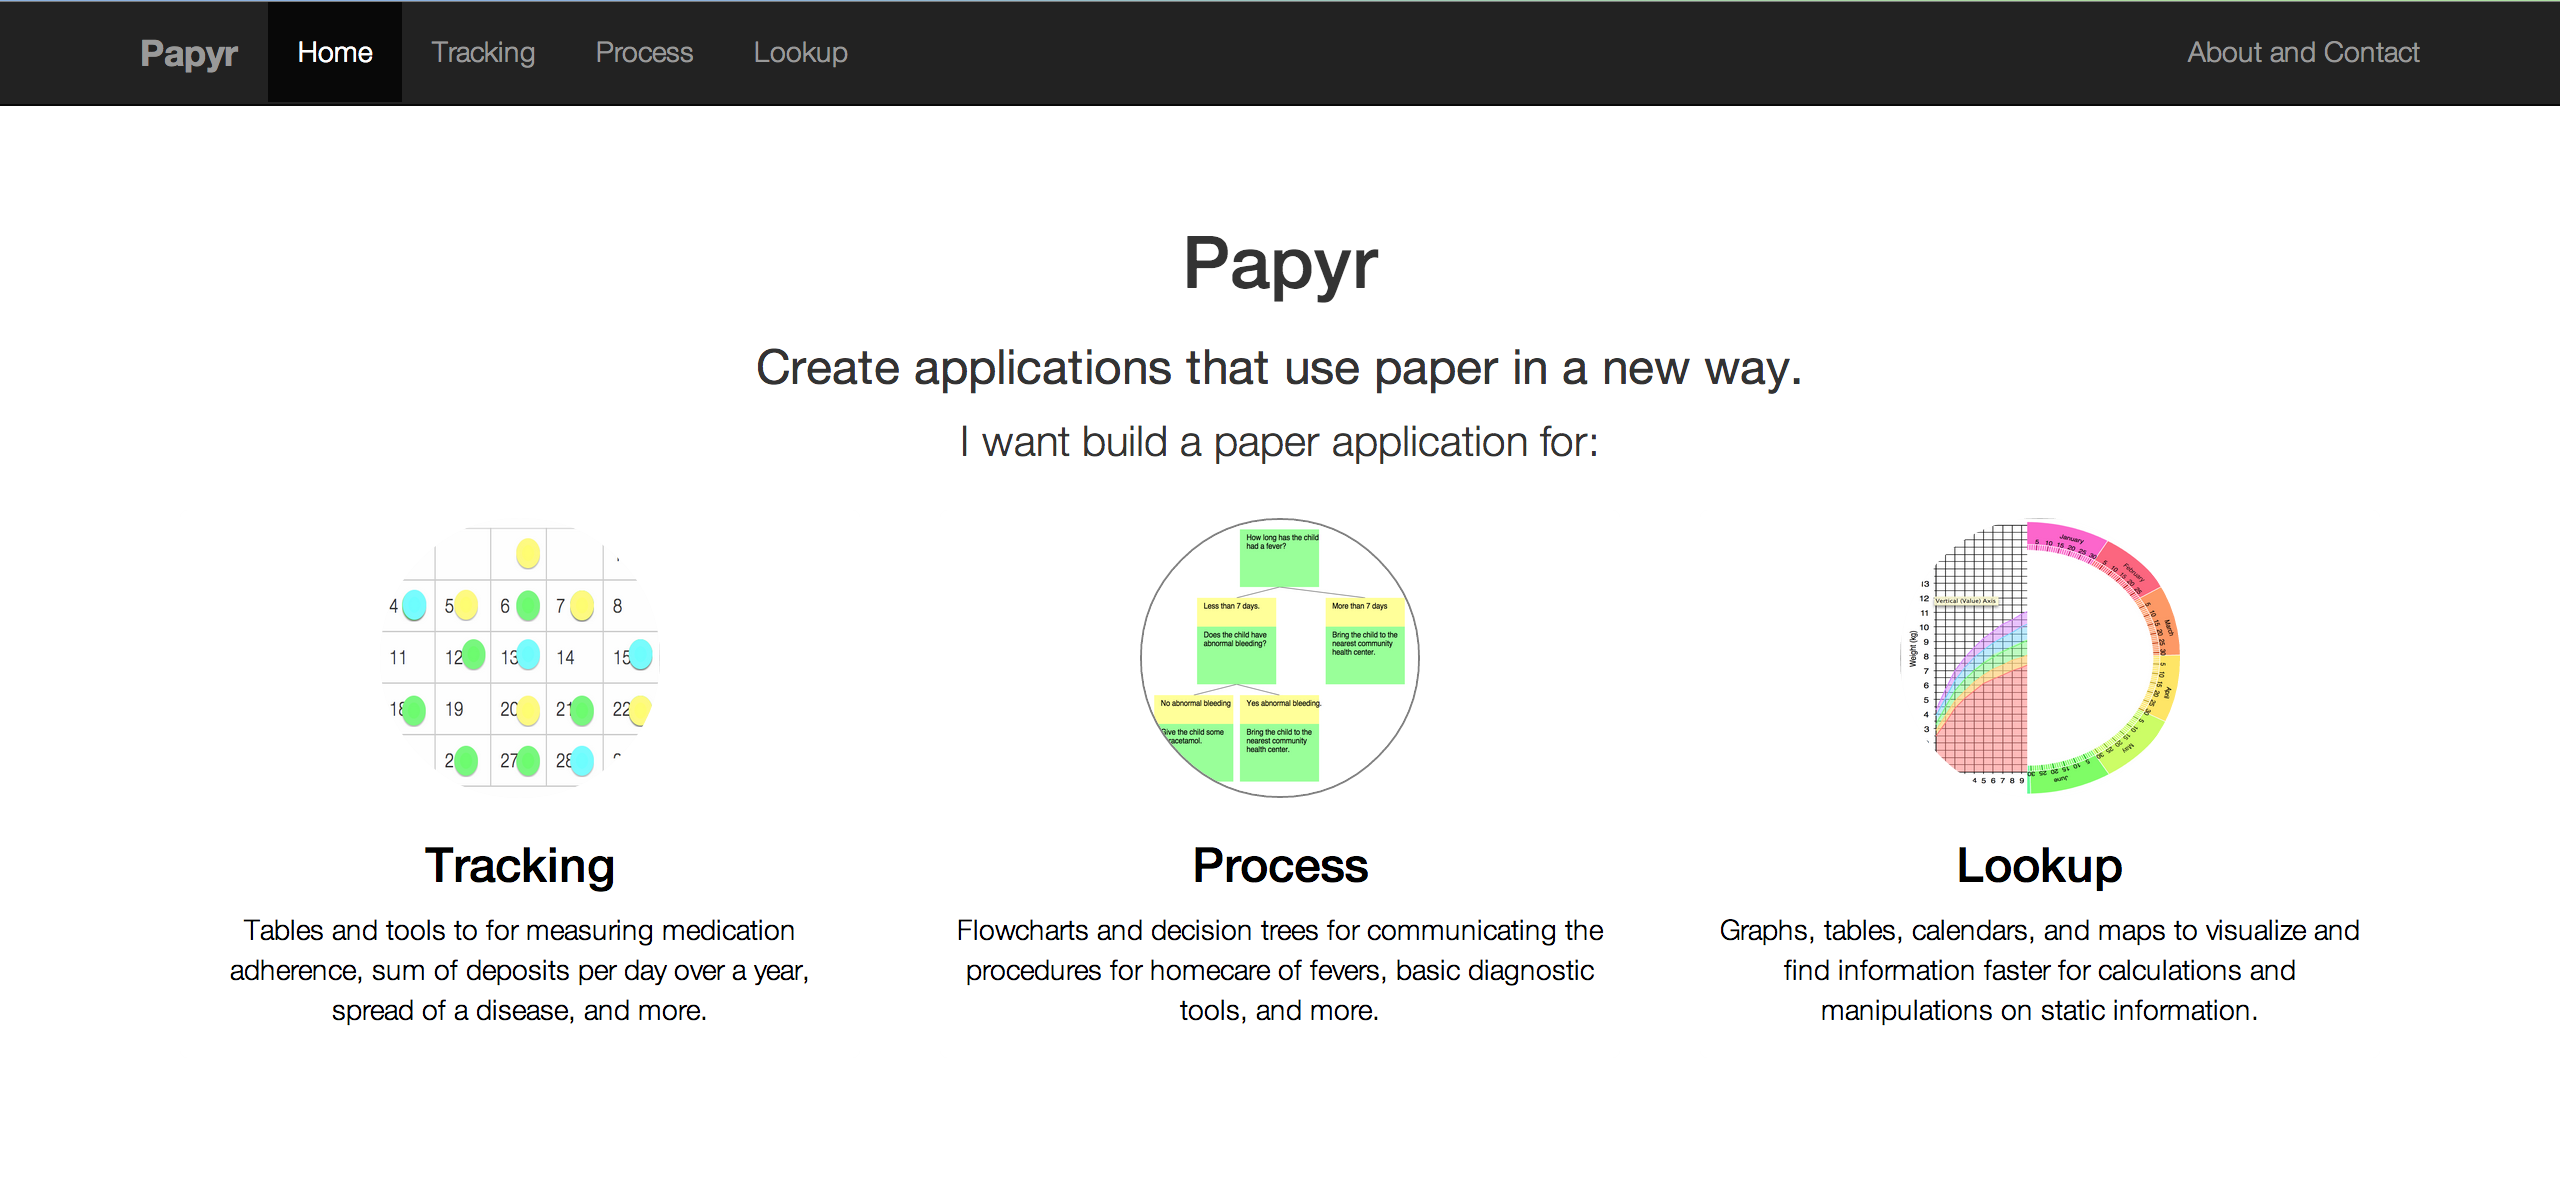
\includegraphics[width=250px]{img/home-screen.png}
% \caption{Screenshot of \nifty interface.}
% \label{fig:home}
% \end{figure}

\subsection{Progress Tracking}
\label{sec:tracking}

\emph{Use cases.}
Tracking encompasses tasks that require periodic user input, including marking the days a patient takes pills to visualize regularity of medication consumption or tracking the days the microfinance savings customer makes the required two cedi deposits to calculate cumulative sum. Other use cases include caloric intake each day over a month, amount of sleep each day, length of menstrual cycle each month, daily journaling or mood tracking, journaling each day, or disease spread throughout a community.

\emph{Task representation.}
% These tasks all have an element of time and the information achieved relies on this element of time. 
In the most basic form, each of these tasks can be done using a table. The main dimension of this table is the change in time, with each row as a single time interval, which varies based on the frequency and the duration for which it is tracked. Another dimension is the values in each one of the cells. Some tasks require only a simple yes or no of whether the event occurred to determine regularity, such as medication consumption, and other tasks require a numeric value that could contribute to a cumulative sum, such as daily deposits.

In the cases where there is more than one piece of data being tracked over time, each task can be defined separately and if the time intervals are compatible, automatically merged into a single table with multiple columns. For example, if the task is to track mood every day, and there are five different possible moods, each of the moods is considered a separate tracking task and merged into a single table with one column for each mood. 
% Users can click a checkbox to disable automatic merging of tasks if this is not desired. 
%There are also cases where location is a factor, such as tracking the occurrence of disease throughout a community. This could be construed similarly as many potential categorizations, tracking the occurrence of disease at each individual locale throughout the community.

%Even complicated examples of tracking tasks could be reduced to this basic tracking over time in a table.

\emph{System implementation.}
One challenge is allowing intermediaries to input task specifications and parameters in an understandable way and to translate this input to paper tool outputs. We originally proposed to allow the intermediary to string together a series of ``per" and ``over" phrases for each relevant time and location to specify their task. For example, an input could read ``I am tracking the regularity of my medication consumption per day over three months." However, this method proves to be ambiguous and difficult for both the intermediary and the computer with more complicated inputs. 

Eventually, the minimal series of questions was developed to elicit the values of the input and the frequency and duration of the tracking. The system is interactive---for each question, \nifty iterates on the intermediary's answers and outputs suggestions, allowing the intermediary to visualize the impact of each additional constraint. For example, after answering the first question, ``What are you tracking?", the intermediary is presented a blank one-column table where only the first row is filled with the task name. The next question asks about the possible values of the tracking task. If the intermediary indicates that they are tracking only whether the event occurs or not, another suggested output is the same one-column table populated with ``YES/NO" in each row so that the end-user can circle the corresponding word based on the occurrence of the event. The intermediary can very clearly see the incremental difference between the blank table and the new ``YES/NO" table when choosing between the two. From there, other options are built such as calendar-based charts for monthly tracking or outcome tallying to count the number of times someone does or does not take their medication. Some examples are seen in Figure~\ref{fig:tracking}.

Each of the output suggestions includes the base table that will be used, as well as a set of possible instructions that vary based on the level of literacy of the end-user and the cost of any external materials. In the previous example, for the blank table, the user receives potential instructions of writing either ``Y" or ``N" on each of the lines depending on whether the event occurs, shading in the rows for the time intervals the event occurs, or placing stickers in those rows.  The intermediary then has the opportunity to compare all of the possible tools along with their associated instructions and select the one that matches their specific context. 

\begin{figure}
\centering
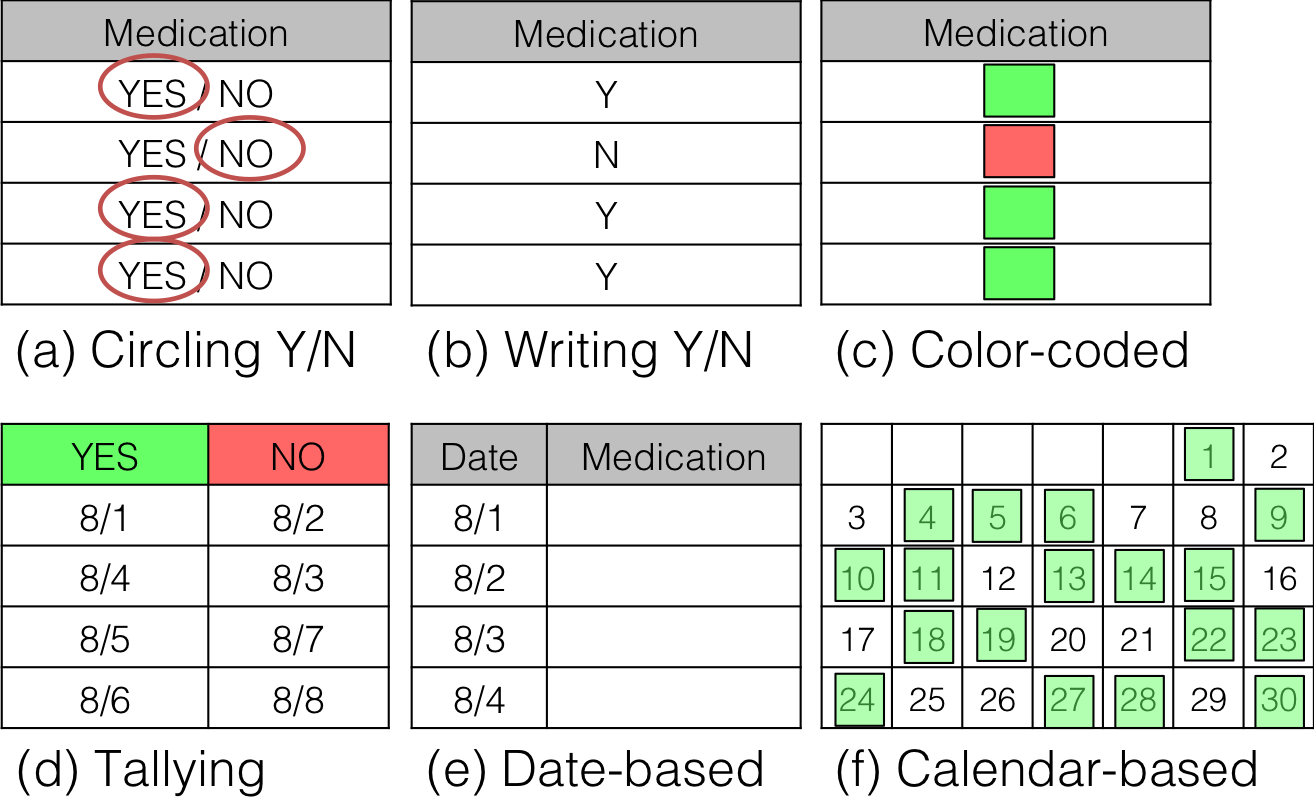
\includegraphics[width=\linewidth]{img/tracking.png}
\caption{\emph{Tracking example (\ref{sec:tracking})}. These are examples of potential outputs by \nifty for tracking whether medication was consumed or not on a daily basis over a month.}
\label{fig:tracking}
\end{figure}

% A screenshot of the \nifty Tracking workflow is seen in Figure~\ref{fig:tracking}. The potential table-based outputs are similar to Figure~\ref{fig:add-init} and Figure~\ref{fig:band-final} for ``sticker with calendar" and ``no sticker with merged tables" outputs respectively.

% For example, if the user wants to track their medication consumption over a month, they would first be asked ``What are you tracking?" They then are prompted to complete the sentence ``I am tracking..." with ``my medication consumption." At this step, the user will be presented with a table one column and only the task name, or ``my medication consumption" as the first row. Then the user is asked to specify what types of input could be given at each point in the process. The types of inputs that the \nifty system currently supports includes tracking occurrence or a single numeric value each time. In the case of medication consumption, the user will specify that they are tracking ``whether the event happens or not" and be presented with a tables that have ``YES / NO" prepopulated for each row. Other outputs would include a two column tally of the number of times the event occurs and the number of times the event does not occur. And if the user had chosen a single numeric value for each time, the rows would be prepopulated with the cumulative sum for each row. Then, the user would be asked about the frequency and duration for which they will be tracking, allowing the tables to have an additional column that would be prepopulated with the time increments the user specifies. And the user would also be presented with a clock or calendar for tracking. This could be that the user will simply mark the times in which the event occurs. Or the user could place a green or red sticker to better visualize regularity.

% The user is first asked ``What are you tracking?" and will answer "I am tracking my medication consumption." This will output a basic empty table with just Then they will be asked to clarify what values this could take on for each time interval, which, in this case, would be whether the event of medication consumption occurred or not. 

% For example, if the user wanted to track their medication consumption over a month, they would first be asked ``What are you tracking?"
%JAY: 2 examples of questions and final outputs
% At each step, \nifty iterates on the user's answers and output suggestions. These suggestions include the base table that will be used, as well as a set of possible instructions that vary based on the level of literacy of the end user and the cost of any external materials. 
% JAY: example of a set of possible instructions

% \begin{figure}
% \centering
% 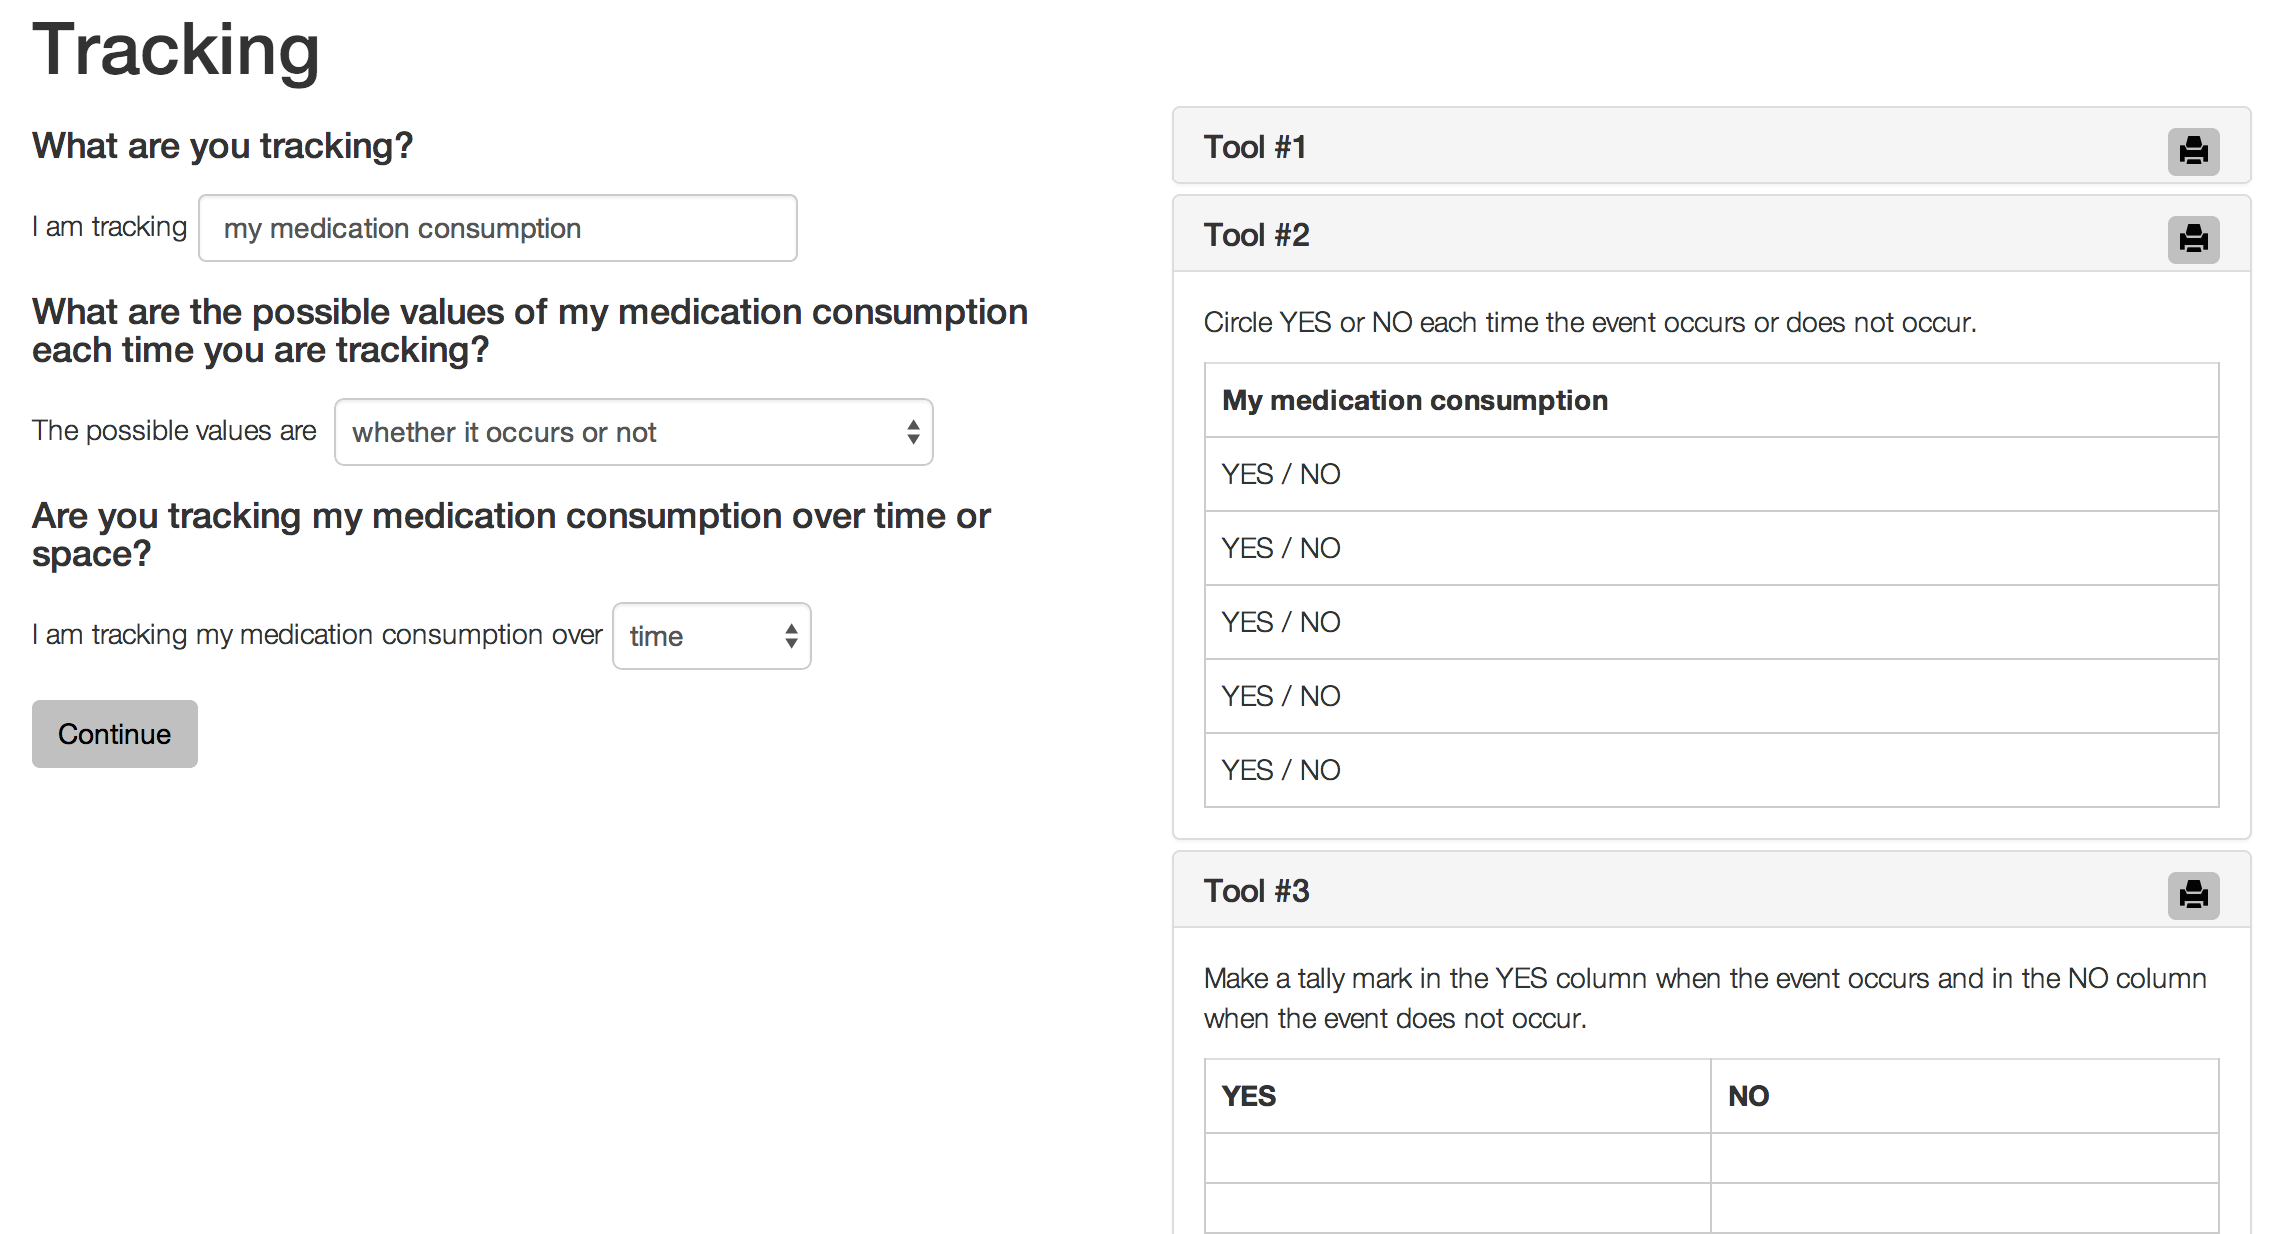
\includegraphics[width=250px]{img/tracking-screen.png}
% \caption{Screenshot of tracking interface.}
% \label{fig:tracking}
% \end{figure}

\subsection{Information Lookup}
\label{sec:lookup}

\emph{Use cases.}
% Information lookup include tasks with static information such as calculating an individual's body mass index (BMI) to looking up whether that BMI falls in the percentiles for being over or underweight or finding out the number of calories for each food item eaten to checking to see if a child's age and weight are at a healthy balance. 
Information lookup includes tasks with static information, such as calculating an individual's body mass index to see if they are over or underweight, finding out the number of calories for each food item consumed, or checking the proper medication dosage given age and weight.

\emph{Task representation.}
All information lookup tasks, calculations included, can be represented as a lookup table. 
% The most common forms of static input and output . Calculations can be construed as information lookups because the answers to a calculation could be enumerated and placed in a lookup table. As with the tracking baseline representation, our baseline representation for lookup is in the form of tables.
The dimensions of these tables are the inputs (i.e. a lookup key) and the outputs (i.e. information the end user is looking up), which are likely numeric or can be reduced to being numerical (i.e. categorical). In the most basic lookup table, all of the inputs are in the first columns and the associated outputs are in the columns that follow (Figure~\ref{fig:table}).

However, there are ways to condense such a large, cumbersome table.
% However, there are many cases in which there are more appropriate ways to represent this data than this large, cumbersome table. 
% In a more specific example, where 
One is when there are two inputs and one output, arranging them so that one input is the columns and the other is the rows and the outputs as the corresponding intersecting cells. In this example, the columns are the weight and the rows are height. If there are two inputs and two outputs, it could be a similar setup but having a color coding for one of the outputs, such as the ``status'' in this example. And if there were more inputs included, such as age in differentiating between adults and children, then the graph can be placed on different pages depending on the third input.

Tables are relatively easy to use for low-dimensional lookups. But with more inputs and outputs, alternative visualizations are beneficial. A clock or calendar could visualize date and time information and a map can be used to visualize geospatial information. Two specialized lookup outputs are graph representations and calendar year calculations.

% In another case where there are potentially three inputs and one output, a similar row-column structure would work for the presentation of two of the three inputs and the final input would be factored into the separation of the table into tables based on different values for that input. And with even larger numbers of inputs, the split could be across different pages, with different colors.

\begin{figure}
\centering
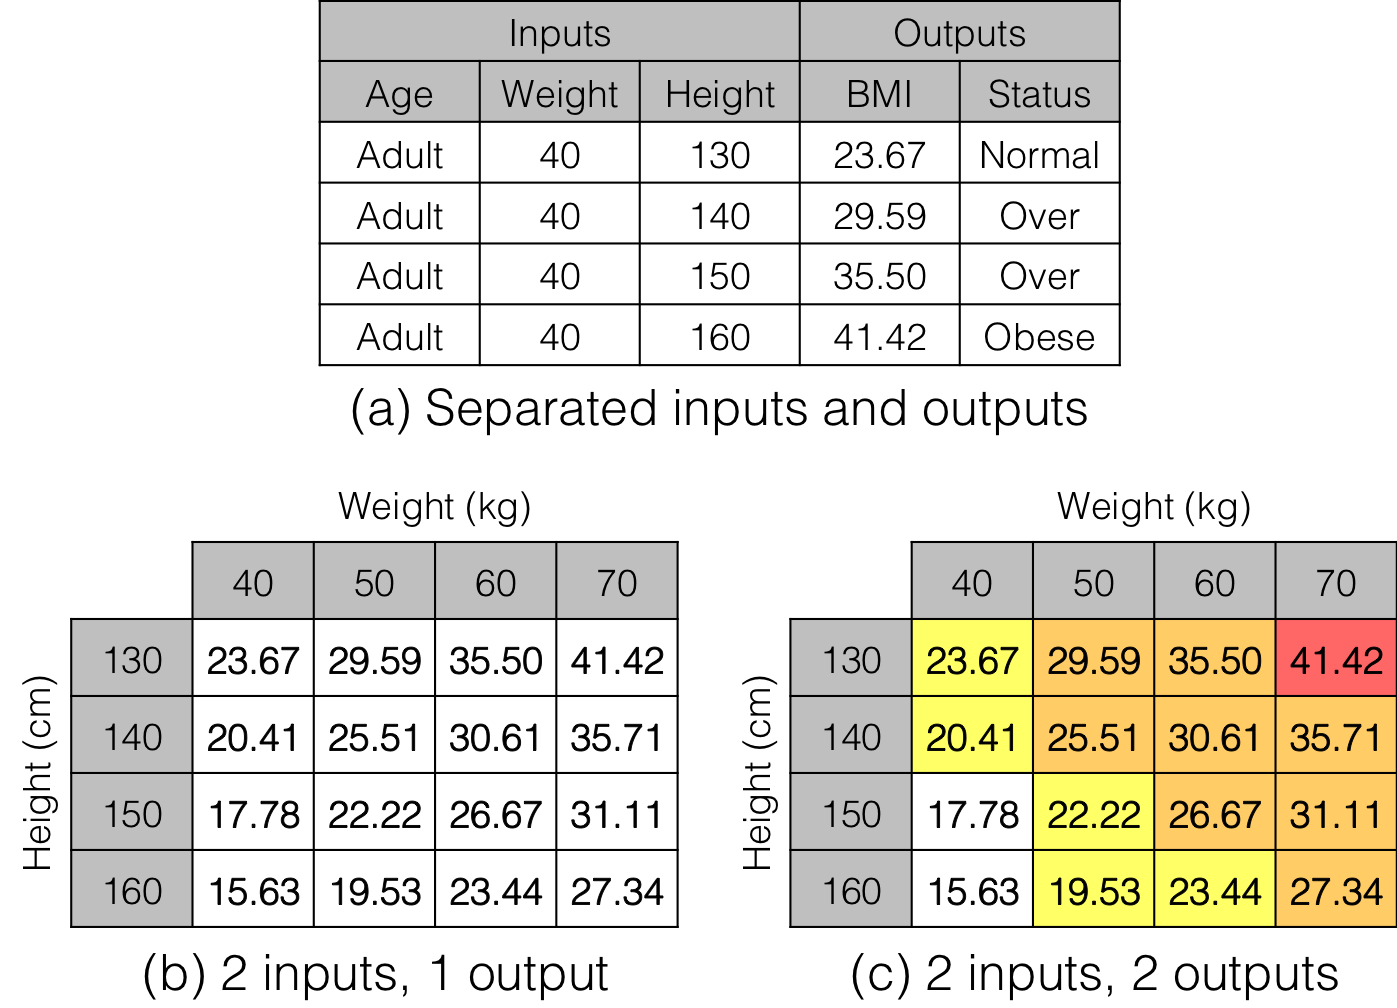
\includegraphics[width=\linewidth]{img/table.png}
\caption{\emph{Lookup table example (Section~\ref{sec:lookup})}. Different table-based representations of lookup tasks with different numbers of inputs and outputs.}
\label{fig:table}
\end{figure}

% \begin{figure}%
%     \centering
%     \subfloat[Basic]{{\label{fig:table-basic}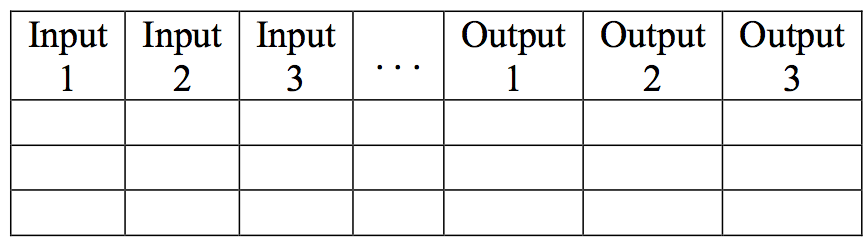
\includegraphics[width=.65\linewidth]{img/table-basic.png} }}%
%     \qquad
%     \subfloat[Two inputs]{{\label{fig:table-inputs}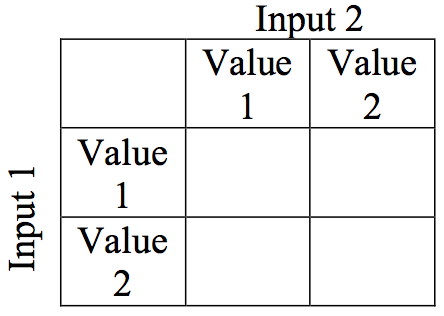
\includegraphics[width=.25\linewidth]{img/table-inputs.png} }}%
%     \qquad
%     \subfloat[Three inputs]{{\label{fig:table-split}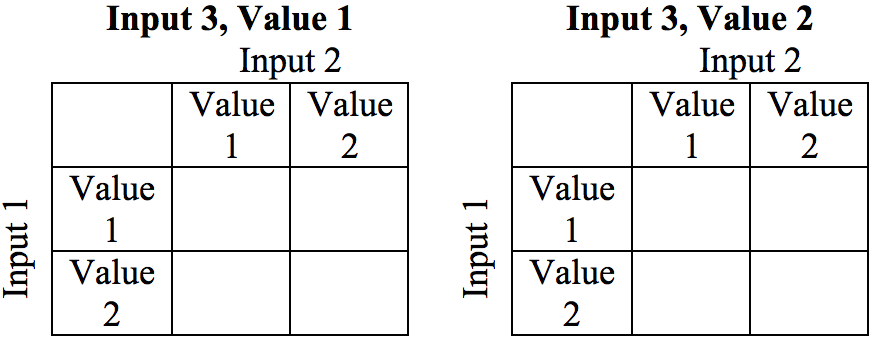
\includegraphics[width=.55\linewidth]{img/table-split.png} }}%
%     \caption{Different arrangements of lookup tables.}%
%     \label{fig:table}%
% \end{figure}

% For low-dimensional lookups, tables are relatively easy to use. For higher-dimensional lookup tasks, alternative visualizations are beneficial. A clock or calendar could be used to visualize time and date information and a map can be used to visualize geospatial information. The two specialized lookup outputs we present here are graph representations and calendar year calculations.

\emph{System implementation.}
% Graph representations cover data that has two numerical dimensions as inputs and a numerical or categorical output. For example, if someone knows their height and weight as numerical inputs, they can figure out whether they fall in the category of under, normal, or overweight based on a graph with those categories as differently colored regions.
Graph representations cover data that has two numerical dimensions as inputs and a numerical or categorical output. The previous BMI example falls in this category. In order to build these graph-based information lookup tools, intermediaries will be asked to input the data that they want to work with, and a graph will be built. Then \nifty will present graph enhancements drawn from the design iterations to help end users with understanding the content of the chart or encourage interactivity. 
The first improvement narrows the end user's focus on the relevant regions of the graph with tabs and cutouts. For graphs with two axes, this is a vertical sliding cover to isolate the y-axis and a horizontal sliding tab to isolate the x-axis. 
% \nifty suggests graph enhancements to help end users with understanding the content of the chart or encourage interactivity. These improvements are drawn from the ideas and feedback collected from the graph reading tool we proposed. The first improvement includes tabs and cutouts to help narrow the end user's focus on the relevant region of the graph. For graphs with two axes, this is a vertical sliding cover to isolate based on the y-axis and a horizontal sliding tab to isolate the x-axis. The user can elect to use these components together or separately. This can be seen in Figure~\ref{fig:graph} which shows the output of a graph tool that has the sliding tabs that pinpoint the relevant information to help block out the rest of the graph. 
A second enhancement is a ``smart viewfinder" that guides the end user in doing basic approximations. For example, sectioning the ``smart viewfinder" into different quadrants determines if the slope of the line from the previous point is positive or negative (e.g. Figure~\ref{fig:graph}). A notched viewfinder could compare the distance between the two points, whether it is comparing the sizes of bars on a bar graph or the amount needed to increase or decrease to be in a different category or region. A copy of output for a printout of the tool is seen in Figure~\ref{fig:graph-print}.

% In order to build these graph-based information lookup tools, users will be asked to input the data that they want to work with, and a graph will be built. Then, users will be presented with the pros and cons of each graph improvement and asked which enhancements they want, whether it is the vertical or horizontal tabs or the viewfinder. 

Calendar year calculations are a specific type of calculation for which there is a tool is made of two concentric circles, the smaller layered on top of the larger. Intermediaries can specify the relative number of days between one event and another, provided the difference is within the 365 day range of a year. Then, by spinning the inner circle to line up with a date on the outer ring, the end user can calculate the date of the next event. For example, gestation occurs approximately 280 days after the last menses. A tool for this aligns the 0 day mark with the date of the last menses, the 14 day mark with conception, and the 280 day mark lines up with the predicted gestation day. This sample tool is seen in Figure~\ref{fig:circletool}. To generate this tool for other calculations, the \nifty system takes as an input an indication of which days are matched with an important event in the year range.

% \begin{figure}%
%     \centering
%     \subfloat[Printed]{{\label{fig:graph-print}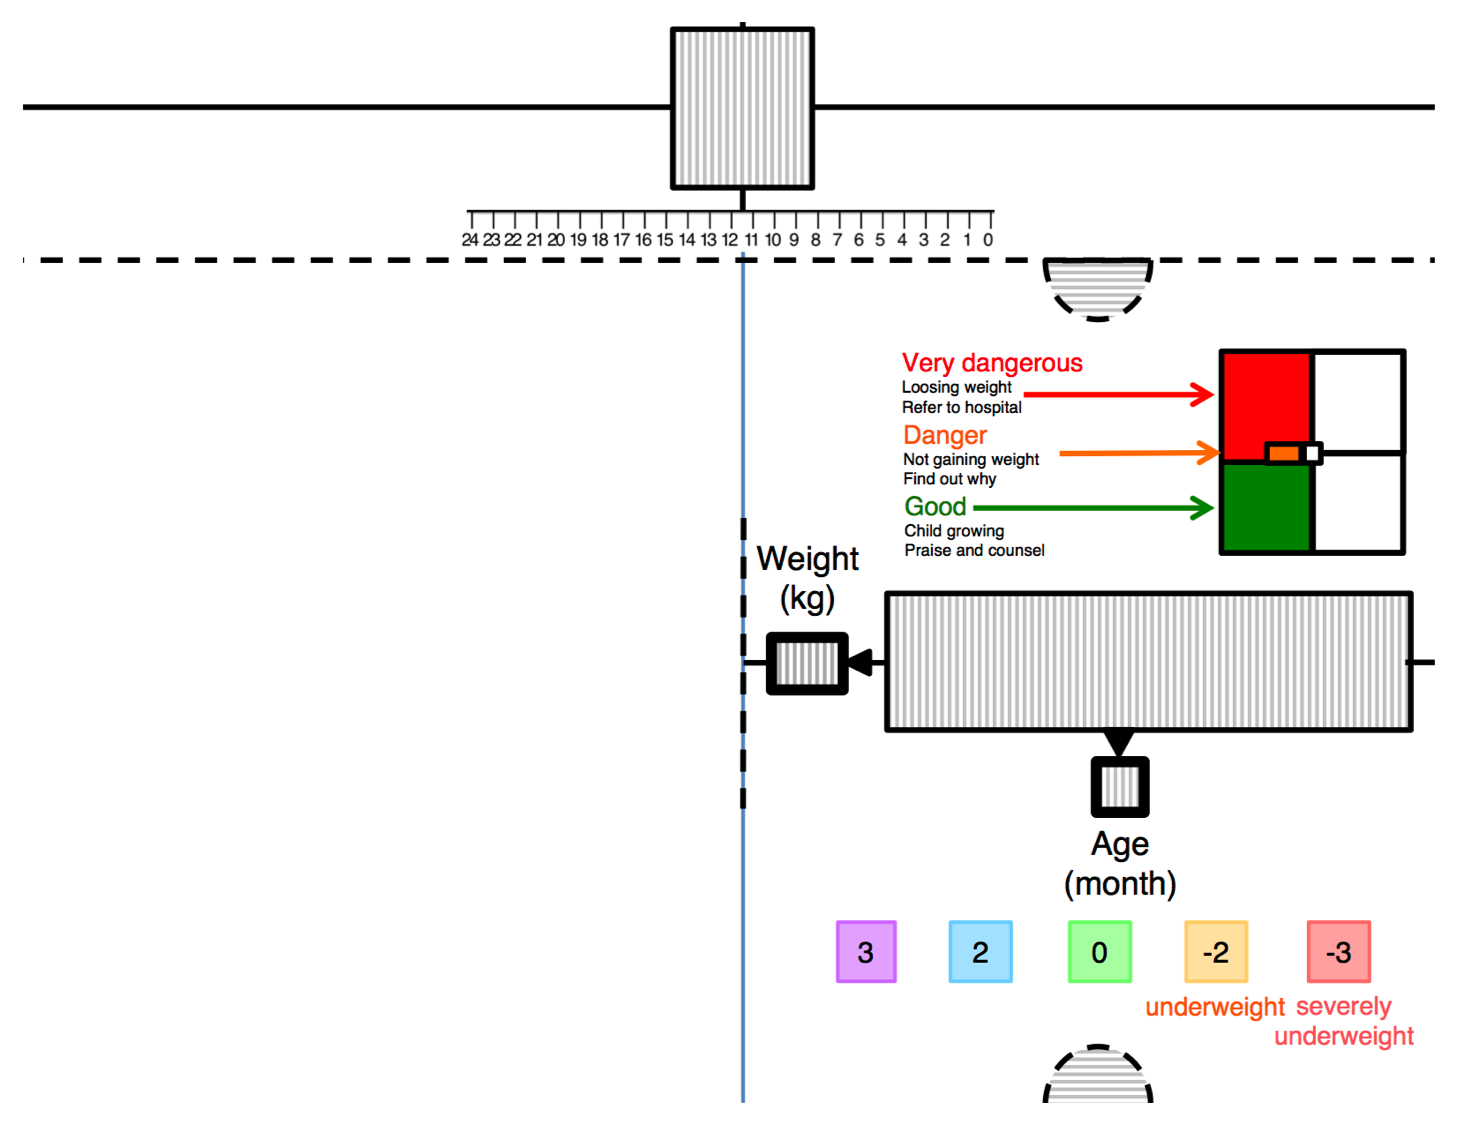
\includegraphics[width=.43\linewidth]{img/graph-print.png} }}%
%     \qquad
%     \subfloat[Assembled]{{\label{fig:graph-tool}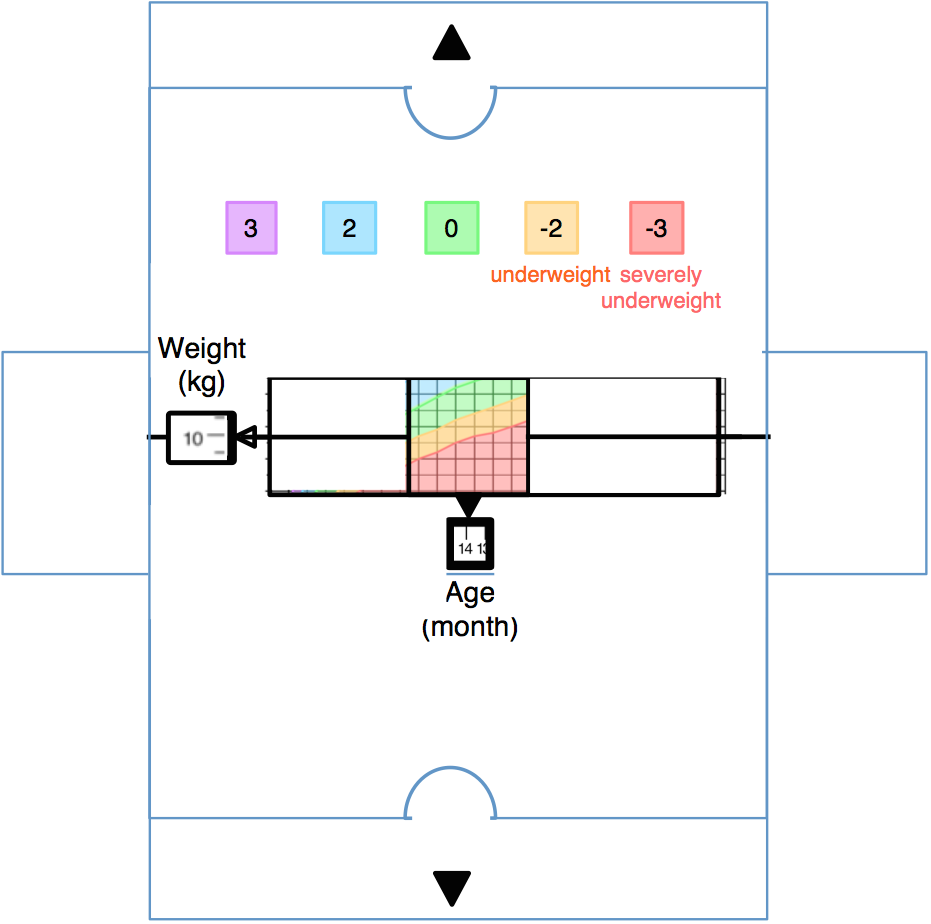
\includegraphics[width=.43\linewidth]{img/graph-tool.png} }}%
%     \caption{Output of the graph generation tool printed and assembled.}%
%     \label{fig:graph}%
% \end{figure}

% \begin{figure}%
%     \centering
%     \subfloat[Printed version of the graph tool with all enhancement. Cut along the dotted lines so that striped sections are removed and fold along the blue line.]{{\label{fig:graph-print}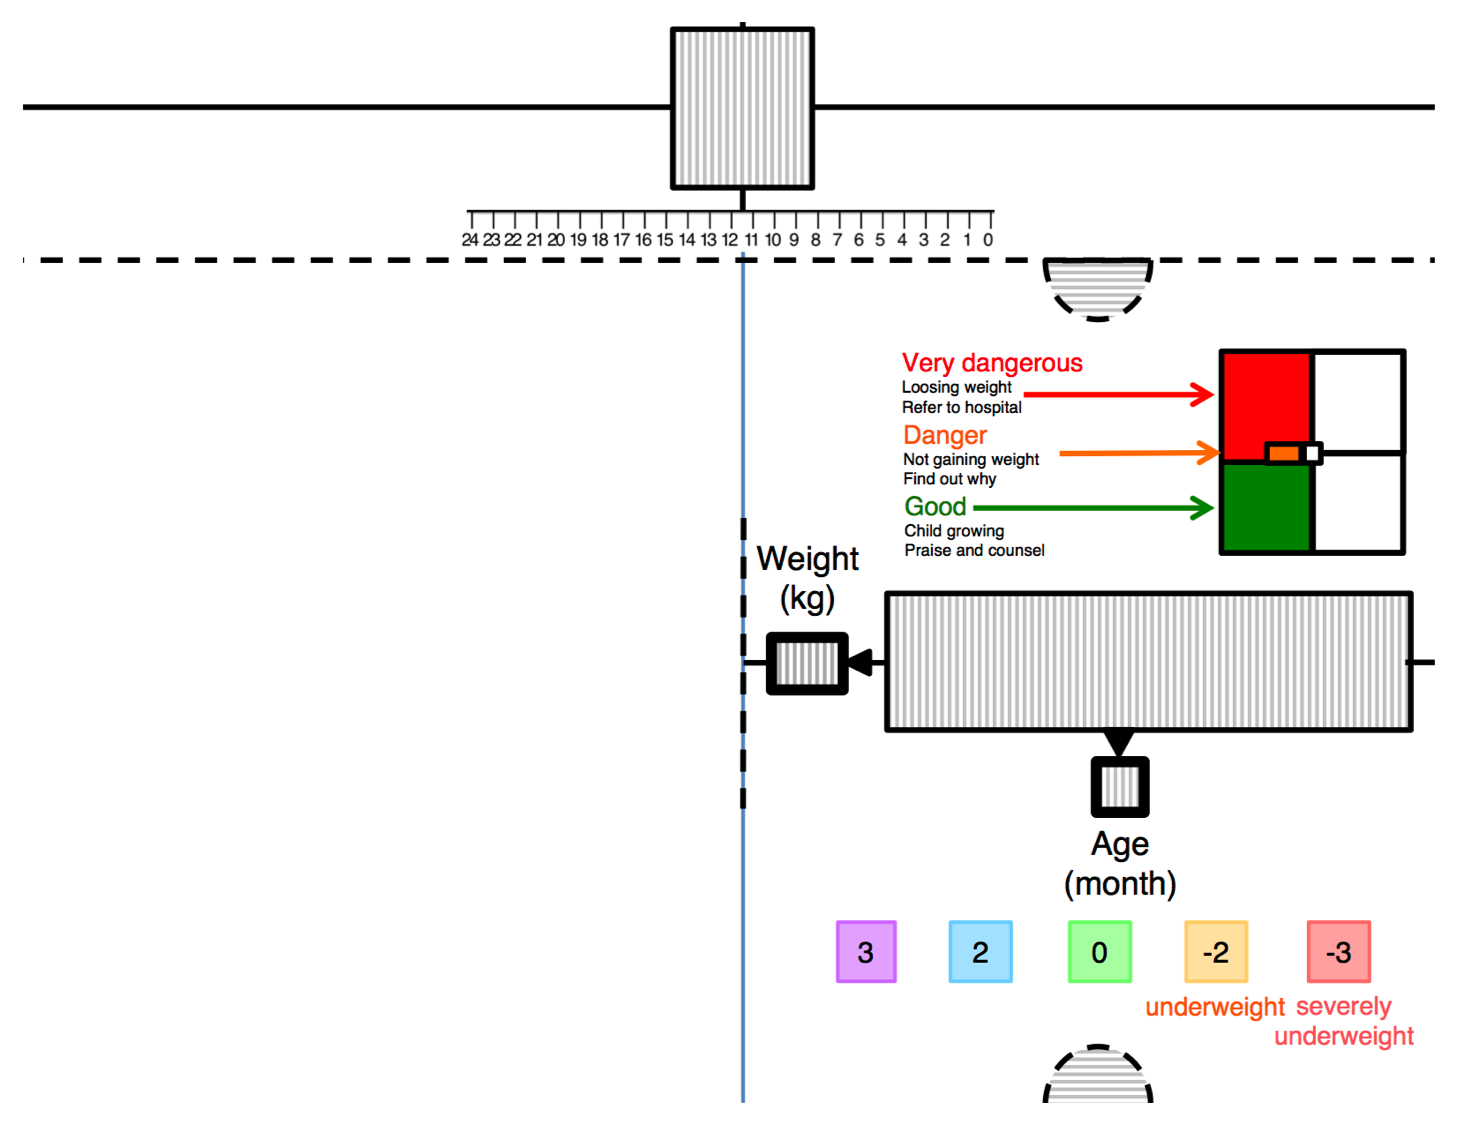
\includegraphics[width=.43\linewidth]{img/graph-print.png} }}%
%     \qquad
%     \subfloat[Printed example of calendar year calculations tool, zoomed in to see the actual interface made of two cocentric circles, where the inner, grey circle is spun so that the red line is spun to the date of last menses.]{{\label{fig:circletool}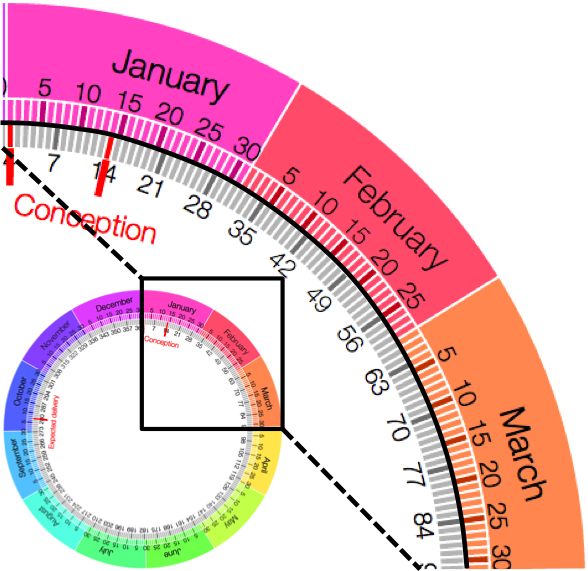
\includegraphics[width=.6\linewidth]{img/circletool.png} }}%
%     \caption{Different outputs from graph module of \nifty (Section~\ref{sec:lookup}).}%
%     \label{fig:lookup}%
% \end{figure}


\begin{figure}
\centering
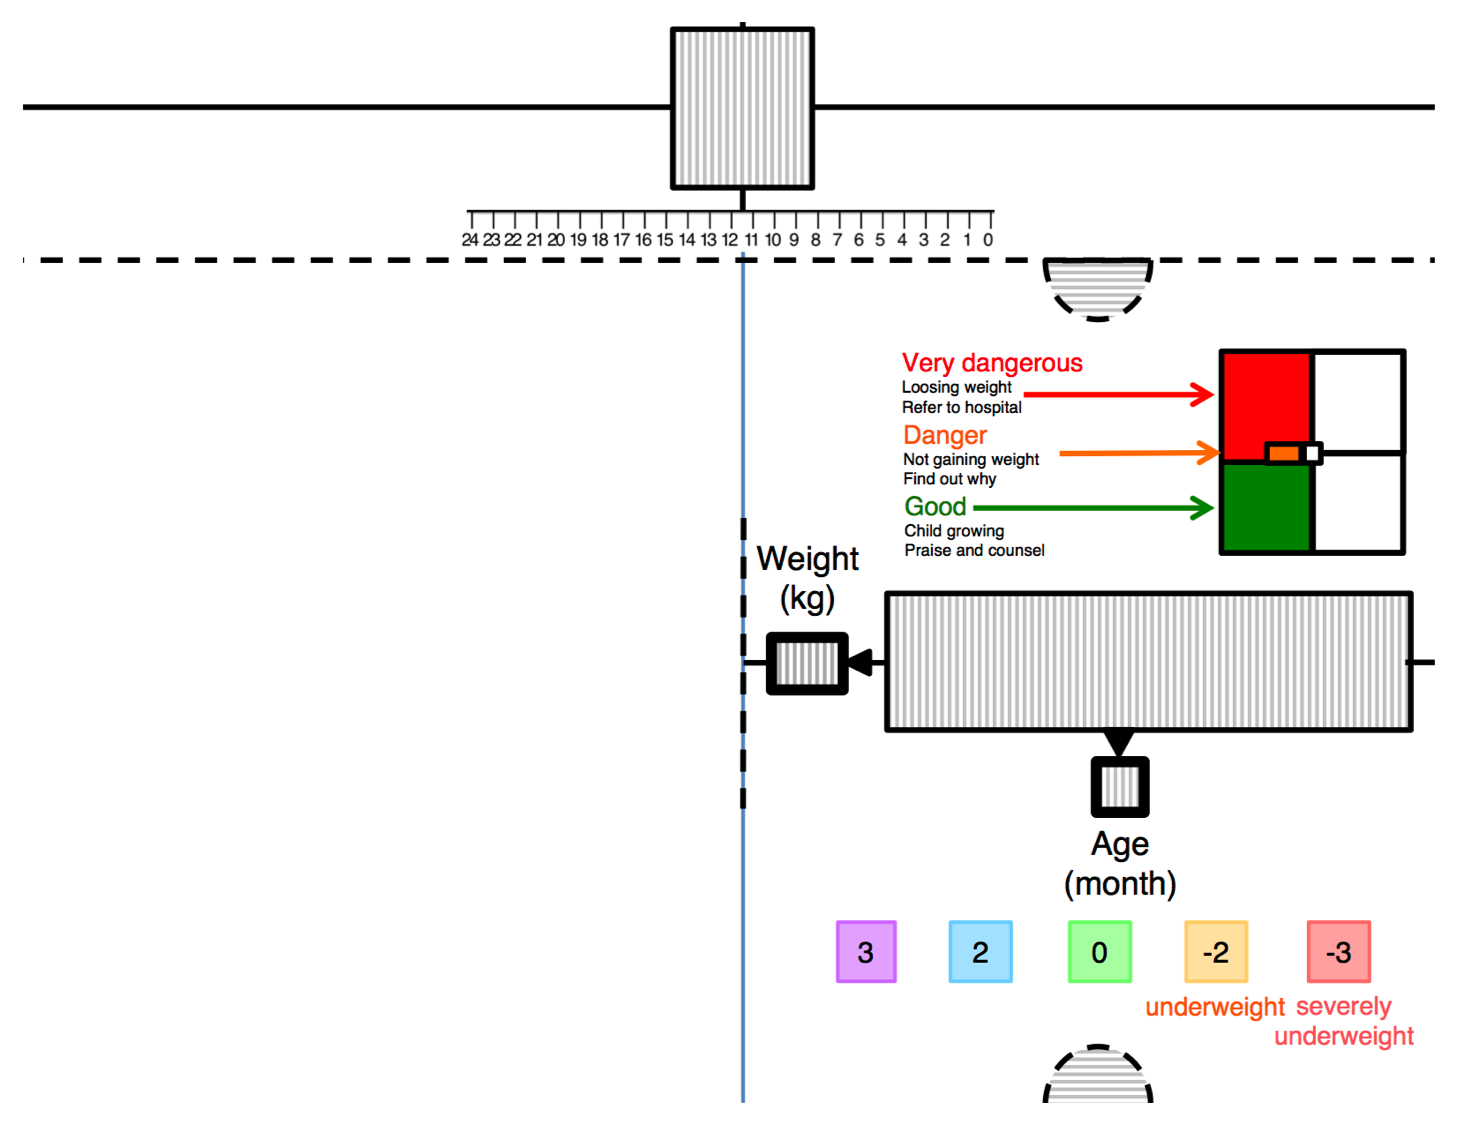
\includegraphics[width=.9\linewidth]{img/graph-print.png}
\caption{Printed output of the graph tool from the lookup module (Section~\ref{sec:lookup}) with all enhancements included. To assemble, cut along the dotted lines so that striped sections are removed and fold along the blue line.}
\label{fig:graph-print}
\end{figure}

\begin{figure}
\centering
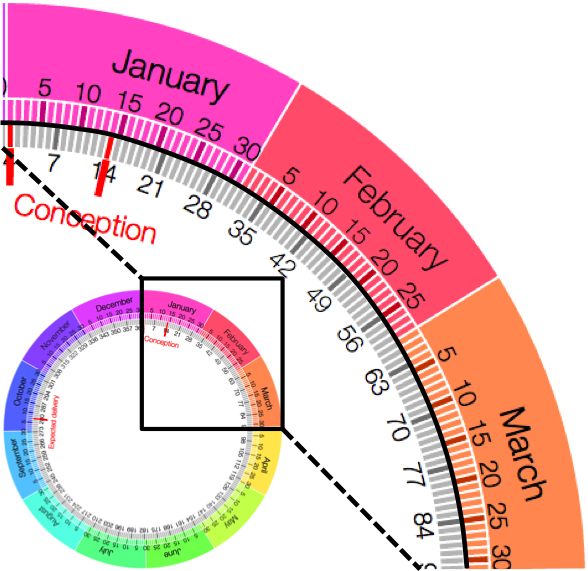
\includegraphics[width=.5\linewidth]{img/circletool.png}
\caption{Printed output of the calendar year calculations tool from the lookup module (Section~\ref{sec:lookup}). The tool can be used by spinning the inner, grey circle so that the red dash lines up with the date of last menses and the conception and gestation markings will line up with the respective, estimated dates.}
\label{fig:circletool}
\end{figure}

\subsection{Decision making}
\label{sec:decision}

\emph{Use cases.}
A specific case of information lookup is decision driven---though it has static information, the relevance of this information depends on the specifics of the situation. Examples include questions community health volunteers use to diagnose a patient, decision diagrams to help a customer choose a savings scheme, or checklists for procedures that change based on the outcome of a step.

\emph{Task representation.}
This information could be presented using a table, with each of the potential factors that contributes to the classification of a given situation as an input and the resulting instructions as an output. However, this results in a fairly sparse table or many sets of sparse tables separated on different pages or sections. More commonly, this type of information is presented in a flowchart or decision tree. 
% The tool produced by the process module of \nifty can be used to depict this logic, including, but not limited to, 

\emph{System implementation.}
In the \nifty system, the intermediary can specify the logic of the process in flowchart form. The flowchart is a directed, acyclic graph whose nodes are the ``steps" or instructions the end user should follow and whose edges are  ``options" or logical connections from one step to another.

For example, if the intermediary is looking to create a tool to help parents with the home treatment of fever in their children, the intermediary first creates a step with the question of ``How long has the child had a fever?" From this question, there are two possible paths that can be taken. The intermediar creates another step connected to the first step with the option ``less than seven days" and the instruction to ``bring the child to the nearest community health center." For the other possible answer to the question, the intermediary creates another step that is connected to the first question with the option ``more than seven days" and with the question ``Does the child have any abnormal bleeding?". The intermediary then continues this process in specifying the answers to this question and continue until no questions remain and all paths end in instruction. This example is presented in Figure~\ref{fig:flowchart-input}.

Then, the system converts this logic into a booklet. Each page of the booklet will present one question from the flowchart and the potential answer options associated with it as tabs below. The end-user can flip the tab over of the option that they select and continue with either the question or the instruction on the page.

Some of the challenges for this workflow in \nifty include the order of the steps and instructions. In order to incorporate the feedback from the needs assessment that there should be no blank pages, balanced with the need to show visible instructions, our algorithm for adapting the process logic from a flowchart to a booklet is a depth first traversal that highlights all nodes, or steps, that are accessed, even those that had been visited before. At each node, the algorithm accesses the children of the node and append these options as tabs at the bottom of the page. If there were no children, append a ``STOP". Another challenge is determining the best way to fit all of the instructions on a page, as per the ``screen real estate" constraint of paper. The default presentation of information is using a fourth of an A4 sheet of paper. However, the intermediary also has the option to adjust the size of each of the pages, which the system uses to parameterize the output.

% \begin{figure}%
%     \centering
%     \subfloat[Flowchart]{{ \label{fig:flowchart-input}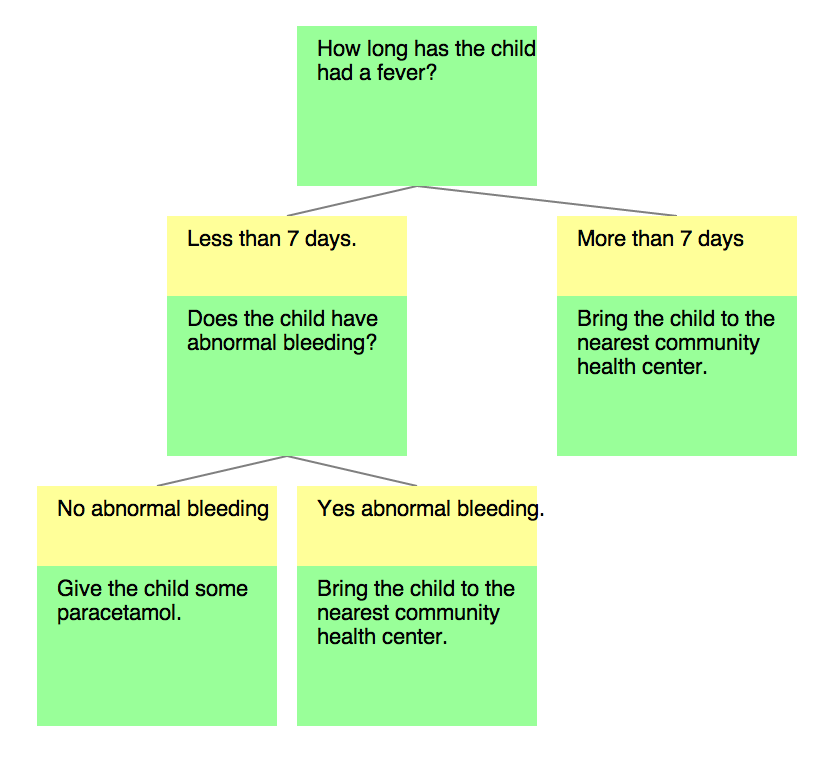
\includegraphics[width=.4\linewidth]{img/flowchart-input.png} }}%
%     \qquad
%     \subfloat[Booklet]{{\label{fig:flowchart-booklet}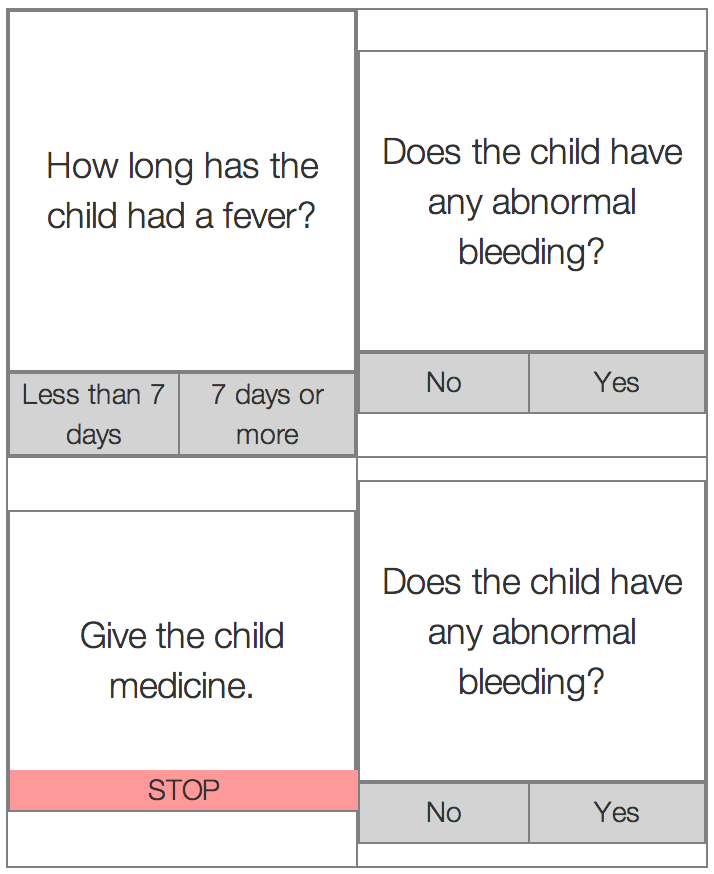
\includegraphics[width=.4\linewidth]{img/flowchart-booklet.png} }}%
%     \caption{Process logic depicted as a flowchart and as a booklet.}%
%     \label{fig:process}%
% \end{figure}

\begin{figure}
\centering
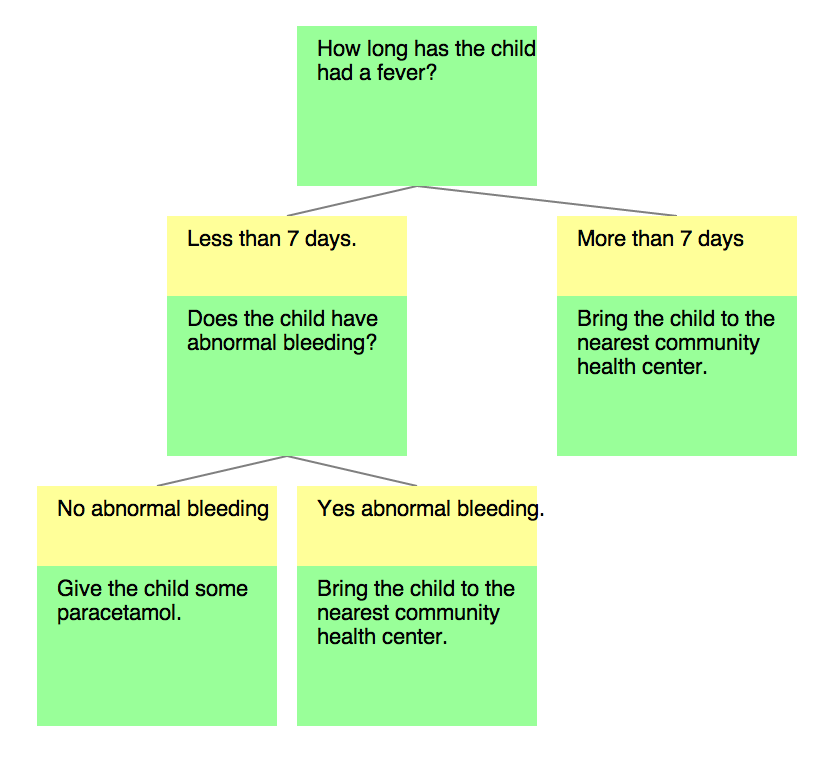
\includegraphics[width=.6\linewidth]{img/flowchart-input.png}
\caption{Example of intermediary input of logic in flowchart format into the decision making module (Section~\ref{sec:decision}).}
\label{fig:flowchart-input}
\end{figure}


% \subsection{Implementation}




%%%%%%%%%%%%%%%%%%%%%%%%%%%%%%%%%%%%%%%%%%%%%%%%%%%%%

\section{Discussion}
\label{sec:discussion}

In abstracting and developing the paper tools and the \nifty system, it was found that the design motivations, principles, and applications remain broadly consistent across all platforms---without considering technology, all the other design considerations remain the same. The same process was followed to test and tweak different iterations of a design and the same questions were asked about user engagement---the results were just slightly different. Therefore, while working within a given degree of computational or visual feedback required to solve a problem, we encourage a more rigorous and dynamic use of paper to resolve some of these problems, especially in low-resource settings.

We believe that the fervent drive to use ICTs to solve a broad range of problems could be scaled back an reconsidered. To avoid the risk of romanticizing paper, we recognize that paper's computational power cannot match that of a computer's. However, paper can certainly be improved over its existing, static uses by integrating more dynamic ``smart'' aspects to it, as we show specifically in the context of low-resource organizations in public health and microfinance. These tools and concepts can easily be abstracted to a host of other applications in the international development space. \nifty uses technology to support the development and creation of paper, unlike existing computing applications that reduce and remove paper's presence by mimicking its properties in a surrogate but ``flashy'' technology artifact. This preserves the affordances of paper for the end user while still being able to accomplish tasks such as progress tracking, information lookup, and decision making. 

\nifty is also unique in its use of intermediaries, such as leaders of microfinance institutions or health officials in a hospital setting, to construct the tools for the end users in a way that is context-relevant. During our time in the field and through our interactions with different users, we discovered that their goals did not always align with the broader goals that we had envisioned for the paper tools. For instance, we assumed that users wanted more complete and precise results what the susu, or savings, tracker was providing them. However, in many cases, users were actually satisfied with or adapted their workflow to the current passbooks. They were able to estimate the approximate cumulative sum based on the number of pages that were filled out and at the time of a withdrawal, many simply asked to withdraw the entire sum of money saved, versus a certain amount. While some of this can be alleviated by retaining some of the original process or look-and-feel of the existing paper tool, as seen in the susu tracking example, this points to the balance between information need and tool ability as well as the general inertia towards the learning and implementation of new tools, paper or otherwise.

In addition to balancing the information needed versus the information that can be provided, there is a tradeoff between information gained and effort exerted. For instance, in the subtraction band, the scattered nature of the sticker sheets, the difficulty of adding and removing stickers, and trickiness associated with the shifting of the band may be disproportionate to the benefit receive, especially when the goal is not precision, but is instead a suitably accurate approximation. This is especially difficult given the extended training of the tool and periodic evaluation and maintenance to ensure that individuals are using the tool properly. Therefore, it is valuable to push the limits of what paper can do, even beyond what we have explored in this paper, to provide the most marginal gain in information possible.

% The motivation driving this study is the fact that paper is abundant, affordable, deeply embedded in existing workflow practices and personal spaces, and familiar, especially when compared to digital devices that are yet to achieve the same level of adoption and use in the developing world. Furthermore, as we demonstrate in this work, paper is capable of providing augmented computational and visual feedback to achieve some of the everyday tasks that computers currently do. Smart paper can perform basic arithmetic tasks, provide regularity and frequency information through visual feedback, and streamline information dissemination. 

% In general, when aiming to solve a problem in a platform-agnostic way (should I use paper or technology?), the design motivations, principles, and applications remain broadly consistent (i.e. without considering technology, all the other design considerations remain the same). Therefore, while working within a given scope, that is the degree of computational or visual feedback required to solve a problem, we encourage a more rigorous and dynamic use of paper to resolve some of these problems, especially in low-resource settings. We believe that the fervent drive to use ICTs to solve a broad range of problems could be scaled back and reconsidered. To avoid the risk of romanticizing paper, we recognize that paper's computational power cannot match that of a computer's. However, paper can certainly be improved over its existing uses as we show specifically in the context of low-resource organizations in public health and microfinance.

% \nifty is a supporting infrastructure that automates the creation of the paper tools. \nifty is unlike existing paper computing applications that almost always reduce paper's presence in these applications, diluting some of its more valuable affordances, or replacing it altogether by mimicking its properties in a surrogate (and ``sexy'') technology artifact. Instead, \nifty leverages technology in the design and creation processes, but the output completely preserves the affordances of paper for the end user.

% During our time in the field and through our interactions with the different users, we also discovered that their goals did not always match the broad goals that we had envisioned for the paper tools. This is not necessarily a user constraint per se, but it did certainly place some checks on the tools we designed and tested in Ghana. For instance, we assumed users wanted more complete and precise results that the susu tracker was providing them. However, in many cases, users were actually satisfied with the current passbooks where they were able to approximate their running total, albeit with some amount of effort. This points to a general inertia towards the learning and implementation of new tools, paper or otherwise. Still, retaining the original look-and-feel of an existing paper tool, something that is more reasonable to accomplish with a new paper tool, like we did with the final iteration of the susu tracker, can help alleviate some of this inertia.

% Some of our more sophisticated tools involved too much effort to use, which did not suitably justify the benefit that users were able to glean from them. For instance, the effort invested in using the subtraction band tool may be disproportionate to the benefit that users receive from the tool, especially when their goal is not precision, but is instead a suitably accurate approximation.
% For similar reasons, while we discussed many paper tool options that would make use of such actions as ripping paper to show approximations, layering paper to demonstrate an increase in magnitude through thickness, or even origami to solve more complex problems, we did not end up designing or iterating on many of these ideas. We limited our \nifty prototype to support only the subset of primitives that we felt confident could be of practical use for health and microfinance problems we encountered.

%To better serve the intended audience for the smart paper tools, that is low-literate populations, we define the user of \nifty to be the intermediaries in a given MFI or hospital or other low-resource organization who are better equipped to define the parameters of the tasks that need to be accomplished, and the specific characteristic of the paper tools that need resolution. Moreover, these intermediaries are more likely to have access to the necessary equipment to be able to use \nifty to generate the paper tools. In this way, we distinctly separate the design, development, and the intended audience for \nifty and the smart paper tools it generates.

%Eventually, this paper encapsulates a three month long process of brainstorming, designing, and developing a paper-technology infrastructure that can support the production and distribution of smart paper tools. 
 
%* Paper is abundant, accessible, familiar in low-resource settings. But drawing on paper by hand, or assembling it by hand is tedious and time-consuming. So we introduced a supporting technology infrastructure. However, we believe in paper's independent qualities, and therefore technology is in the picture only up to the point of distribution. 

%* Intermediary uses Nifty Paper, end-user uses the paper tools

%*We demonstrate paper's ability to provide augmented computational and visual feedback. Paper's potential still untapped. Insert commentary about paper's "dimensions"

%* Don't want to romanticize paper. Yet want to make a normative call against productizing at the drop of a hat. Technology does not solve all problems, and going through a resource-intensive process to discover this may be futile. Instead try with paper tools! Insert commentary about how the design process for smart paper tool and technology tools are similar, especially when they are solving the same problem.

%JAY: something about the design space
% Through the survey of existing tools and brainstorming potential tools that push the boundaries of paper, we have discovered some of the principles of designing ``smart" paper tools. 

%JAY: Something similar to this here to contrast again with related work. In contrast,this project focuses instead almost exclusively on exploitingand preserving the valuable affordances of paper by bring-ing in technology to furnish thesupportinginfrastructure togenerate smart paper tools

%%%%%%%%%%%%%%%%%%%%%%%%%%%%%%%%%%%%%%%%%%%%%%%%%%%%%

% \section{Conclusions}

%%%%%%%%%%%%%%%%%%%%%%%%%%%%%%%%%%%%%%%%%%%%%%%%%%%%%

\section{Conclusions and Future Work}
\label{sec:future-work}

The motivation driving this study is the fact that paper is abundant, affordable, more familiar than technological devices, and deeply embedded in existing workflow practices and personal spaces. This paper describes an exploration into the design of ``smart'' paper tools, or using paper to provide augmented computational and visual feedback to achieve some of the arithmetic tasks, regularity visualization, and information dissemination that computers currently do. We describe the process of brainstorming, designing, assessing, and developing a paper-technology infrastructure that automates the production and distribution of smart paper tools in low-resource settings: we explore existing paper tools in healthcare and microfinance in Ghana, we iterate on several potential designs of enhanced paper-based tools that push the boundaries of paper, and we design a smart paper generation tool, \nifty, that allows intermediaries to specify tasks to quickly and automatically customize potential paper-based solutions that do not require ICTs at the point of use. \nifty can be used to produce smart paper tools that preserve the affordances of paper for the end user.

There are many ways this work can be extended with regards to the exploration of the capabilities of paper. There are various primitive actions that can be done onto paper that were not included in this study, including, but not limited to, ripping, stacking, layering, or complex folding (origami) with paper. This could result in understanding how layering could help figure out clustering of disease incidence across households in a community or incremental folding of different shapes could  tracking. Looking at other low-cost materials, it is interesting to explore the properties of these items as well or look at ways to create composites with paper to explore more of the spectrum between paper and technology.

Furthermore, there are many ways the project can be extended with the development of the \nifty system including improvements to specific modules or expansion of the overall capabilities. Future iterations can include more specialized tools such as maps for geospatial events in progress tracking or editable calendars for information lookup. Another step includes the support for uploading images or different languages to help adjust the application to be more inclusive over different languages and literacy-levels. We plan to provide \nifty as a free open-source platform for immediate use by low-resource organizations.

% This paper describes the an exploration into the design of ``smart'' paper tools in the context of developing regions. We described the process of brainstorming, designing, assessing, and developing a paper-technology infrastructure that automates the production and distribution of smart paper tools. We explored existing paper tool use in healthcare and microfinance in Ghana to understand how paper is currently being used by low-resource organizations to track and disseminate information. From our needs assessment we iterated on several potential designs of enhanced paper-based tools to push the boundaries of paper. We designed a smart paper generation tool that allows intermediaries to specify tasks to quickly and automatically construct potential paper-based solutions that do not require ICTs at the point of use. We describe the design and implementation of our ``smart paper'' prototype, \nifty and demonstrate how it can be used to produce smart paper outputs that preserve the affordances of paper for the end user.

% The motivation driving this study is the fact that paper is abundant, affordable, deeply embedded in existing workflow practices and personal spaces, and familiar, especially when compared to digital devices that are yet to achieve the same level of adoption and use in the developing world. Furthermore, as we demonstrate in this work, paper is capable of providing augmented computational and visual feedback to achieve some of the everyday tasks that computers currently do. Smart paper can perform basic arithmetic tasks, provide regularity and frequency information through visual feedback, and streamline information dissemination.



% There are many features that we are still incorporating into \nifty and even more areas of improvement. We believe that there is ample potential to leverage paper's tangibility in future work. We plan to explore many of the ideas we mentioned here including: ripping, stacking, layering, or complex folding (origami) with paper. There is also potential to improve the specific modules in \nifty. For instance, future iterations of the tracking workflow will include improved abstractions and optimizations from the given tables, so as to better handle more inputs across different tasks, including optimizations of using maps to track the events across geographical space. In the same vein, future versions of the information lookup workflow will produce more specialized tools including editable calendars and maps. Finally, a future optimization on process streamlining will allow the inclusion of images as components of the steps, for both the questions as well as the instructions and options to better accommodate low-literate individuals. We plan to provide \nifty as a free open-source platform for immediate use by low-resource organizations.

% The mot






%%%%%%%%%%%%%%%%%%%%%%%%%%%%%%%%%%%%%%%%%%%%%%%%%%%%%

\section{Acknowledgements}
% We would like to thank all of those who gave us valuable feedback and support along the way.
We thank the participants of our studies for their patience, helpfulness, and valuable feedback.
% We thank David Hutchful at Grameen Foundation for his valuable assistance on the ground.
% We thank the people we interviewed and who helped give us feedback (?)
% Also, how would you even "deeply thank" someone?

%%%%%%%%%%%%%%%%%%%%%%%%%%%%%%%%%%%%%%%%%%%%%%%%%%%%%
\bibliographystyle{abbrv}
\bibliography{ref}

\end{document}